L'objectif premier des observations d'amas de galaxies avec NIKA2 est de mesurer les propriétés thermodynamiques du milieu intra-amas.
En particulier, l'amplitude du signal tSZ mesuré en direction d'un amas permet la mesure de sa distribution de pression, qui peut ensuite être combinée à des observations X pour estimer la distribution de masse de l'amas, ainsi que d'autres propriétés thermodynamiques, comme décrit en section \mypageref{sec:lpsz_sci}.

Le logiciel \texttt{PANCO} (\textit{Pipeline for the Analysis of NIKA2 Cluster Observations}) développé par F. \myciteauthor{ruppin_cosmologie_2018} a pour objectif d'automatiser ce processus dans le contexte du grand programme SZ de NIKA2.
Au cours de ma thèse, après avoir utilisé ce logiciel, j'ai décidé d'en développer une version plus optimisée, basée sur l'utilisation de librairies Python dédiées au calcul numérique.
L'objectif de ce développement était double.
D'une part, il était nécessaire de fournir à la collaboration NIKA2 un code plus rapide, le temps d'exécution de \texttt{PANCO} étant trop grand pour permettre l'analyse d'échantillons d'amas.
D'autre part, il s'agissait d'une occasion de créer un outil standard pour le grand programme SZ de NIKA2, là où \texttt{PANCO} avait été développé pour l'analyse jointe de plusieurs cartes d'un même amas.

Ce nouveau logiciel, nommé \texttt{PANCO2}, a été rendu disponible pour la collaboration NIKA2, après avoir été testé sur des simulations.
Le temps d'exécution a été réduit d'un facteur dix à cent par rapport à \texttt{PANCO}.
Ce gain en performance a motivé le choix de \texttt{PANCO2} comme pipeline SZ officiel de la collaboration NIKA2.
Une généralisation du code est en cours, qui permettra d'utiliser \texttt{PANCO2} pour l'exploitation de cartes issues d'autres instruments, et qui sera livrée à la communauté comme un code public.
Ce chapitre décrit \texttt{PANCO2}, du principe de la mesure des propriétés thermodynamiques de l'ICM grâce à l'effet SZ à l'algorithme employé pour effectuer cette mesure.

\begin{figure*}[t]
    \centering
    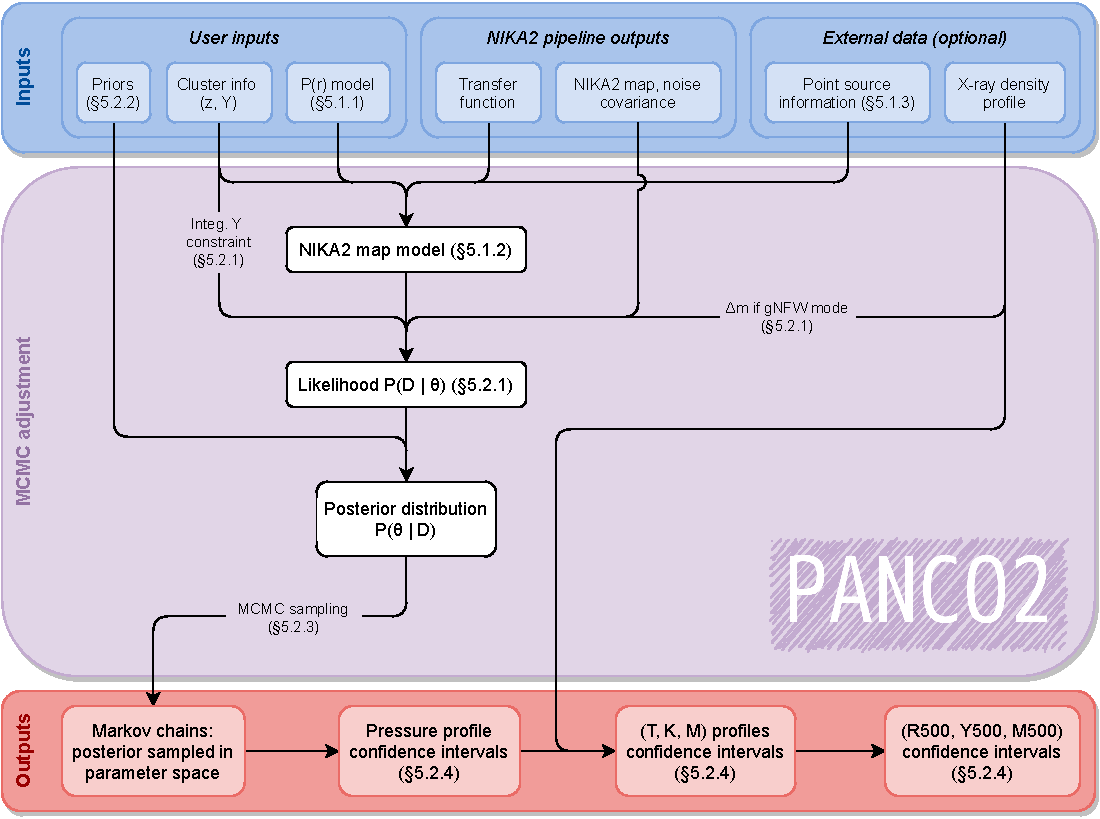
\includegraphics[width=.9\linewidth]{Figures/Chap_panco/panco2_workflow.pdf}
    \caption{
        Schéma représentant le principe de fonctionnement de \texttt{PANCO2}.
        Les données d'entrée sont les produits standards pour les observations NIKA2 d'amas de galaxies, produits par le pipeline d'analyse des données brutes présenté au chapitre \ref{chap:decorr}, ainsi que des données externes telles que les profils radiaux mesurés en X ou les informations sur les sources ponctuelles.
    }
    \label{fig:panco:schema}
\end{figure*}

Un schéma synoptique du fonctionnement de \texttt{PANCO2} est présenté en figure \ref{fig:panco:schema}.
Il répertorie les différentes données d'entrée (bleu) nécessaire à la mesure des propriétés thermodynamiques (rouge).
Les données principales sont les sorties du pipeline de la collaboration NIKA2, décrites au chapitre précédent.
Des informations sur la contamination par des sources ponctuelles, issues du logiciel \texttt{PSTools} détaillé en section \ref{sec:decor:pstools}, peuvent également être fournies -- elles seront discutées en \mypageref{sec:panco_ps}.
On note aussi la possibilité de donner en entrée un profil de densité mesuré en X, qui permettra la combinaison des données X et SZ pour une caractérisation détaillée des propriétés thermodynamiques du milieu intra-amas, discutée en \ref{sec:panco:thermo}.

% ==================================================================================== %
\section{Modélisation du signal SZ}

L'objectif principal de \texttt{PANCO2} est la mesure du profil de pression du milieu intra-amas à partir d'une carte de l'effet SZ.
Pour cela, une approche \textit{forward modelling} est employée.
Une modélisation de l'état physique du système, basée sur un nombre de paramètres, est établie, puis affectée des différents effets ayant donné naissance aux données observées.
Cela permet dans notre cas d'obtenir, à partir d'hypothèses physiques, un modèle de l'effet SZ mesuré par NIKA2, qui sera comparé aux données afin d'estimer les propriétés physiques de l'amas.
Cette section décrit les étapes successives nécessaires à l'obtention d'un tel modèle.

% ------------------------------------------------------------------------------------ %
\subsection{Profil de pression et effet Sunyaev-Zeldovich} \label{sec:panco:p_prof}

Comme décrit dans le chapitre~\ref{chap:amas}, l'effet Sunyaev-Zeldovich est une distorsion spectrale du fond diffus cosmologique due à la diffusion Compton inverse des photons sur les électrons du milieu intra-amas.
Dans le cadre de l'effet Sunyaev-Zeldovich thermique, dominant dans les observations NIKA2 d'amas de galaxies, l'énergie transférée par les électrons provient de leur grande agitation thermique.
L'amplitude de la distorsion observée aux coordonnées $\theta$ est alors appelée paramètre de Compton $y$, et est proportionnelle à la pression électronique $P_\e$ du milieu intra-amas intégrée le long de la ligne de visée (LdV) correspondante.
D'après l'équation (\ref{eq:sz_y}, page \pageref{eq:sz_y}), on a:
\begin{equation}
    \label{eq:panco:y_los}
    y(\theta) = \frac{\sigma_\textsc{t}}{m_\e c^2} \int_{\rm LdV(\theta)} P_\e(l) \; \d l .
\end{equation}

Par conséquent, la cartographie de l'effet SZ est une mesure directe de la distribution intégrée de pression du milieu intra-amas dans le plan céleste.
Bien que cette distribution ne soit pas mesurable le long de la ligne de visée, des hypothèses peuvent être faites sur la symétrie du milieu intra-amas.
Dans le cadre de l'hypothèse de symétrie sphérique, la distribution de pression ne dépend que de la distance au centre de l'amas, et est alors décrite par un profil radial de pression $P_\e(r)$.
Une carte de l'effet tSZ permet alors de contraindre ce profil de pression.
Par transformation d'Abel, l'équation (\ref{eq:panco:y_los}) devient:
\begin{equation}
    \label{eq:panco:y_abel}
    y(R) = 2\frac{\sigma_\textsc{t}}{m_\e c^2} \int_{R}^{+\infty} \frac{r}{\sqrt{r^2 - R^2}} \; P_\e(r) \; \d r .
\end{equation}

L'objectif principal de \texttt{PANCO2} est la mesure du profil de pression dans l'hypothèse de symétrie sphérique.
Dans \texttt{PANCO2}, je propose deux modélisations du milieu intra-amas, illustrées sur la figure \ref{fig:panco:gnfw_np}:
\begin{itemize}[leftmargin=*]
    \setlength\itemsep{5pt}
    \item Le modèle Navarro-Frenk-White généralisé (noté \guillemotleft gNFW \guillemotright), dans lequel le profil de pression est décrit par \cite{zhao_analytical_1996,nagai_effects_2007} :
    \begin{equation}
        \label{eq:panco:gnfw}
        P_\e(r) = P_0
        \left(\frac{r}{r_{\rm p}}\right)^{-c}
        \left[1 + \left(\frac{r}{r_{\rm p}}\right)^a \right]^\frac{c-b}{a} ,
    \end{equation}
    où $P_0$ représente la normalisation du profil, $b$ et $c$ les pentes externe et interne du profil de pression, et $r_{\rm p}$ et $a$ le rayon de transition entre les deux régimes et le caractère abrupt de cette transition;

\item Un modèle dit \guillemotleft non-paramétrique\footnotemark\guillemotright, dans lequel le profil de pression est décrit par des coquilles sphériques concentriques au sein desquelles la pression diminue avec le rayon en loi de puissance selon \cite{ruppin_non-parametric_2017,romero_multi-instrument_2018}:
    \begin{equation}
        \label{eq:panco:nonparam}
        P_\e(r) = P_i \left(\frac{r}{R_i}\right)^{-\alpha_i} .
    \end{equation}
\end{itemize}
\footnotetext{Il serait plus juste de parler de profil \guillemotleft binné \guillemotright, car le modèle est de fait paramétrique: ses paramètres sont les valeurs du profil de pression aux rayons spécifiés. Nous parlerons toutefois de modèle non-paramétrique par abus de langage, et par opposition au modèle gNFW dans lequel le nombre de paramètres est fixé par l'expression du modèle.}

Chacune des modélisations présente ses avantages et inconvénients.
Le profil gNFW est une fonction continue du rayon, aisément extrapolable et avec un nombre fixe de paramètres, le rendant plus directement comparable à la littérature dans laquelle il est le plus répandu.
Le profil non-paramétrique offre quant à lui une approche moins dépendante du modèle, et donc la possibilité de détecter des irrégularités dans le profil de pression, telles que des régions de surpression locales dues par exemple à des chocs.
Le plus grand avantage du profil non-paramétrique provient cependant des corrélations plus faibles entre ses paramètres, qui offre de meilleures performances dans l'ajustement, comme décrit dans la section \mypageref{sec:music_pressure}.

\begin{SCfigure*}[][t]
    \caption{
        Comparaison entre un profil de pression gNFW (bleu) et non-paramétrique (rouge).
        La valeur de la pression du profil non-paramétrique est divisée par deux à des fins de visibilité.
        Les lignes pointillées représentent l'extrapolation du profil non-paramétrique au-delà du premier et dernier point, en considérant une loi de puissance identique à celle entre le premier et deuxième point (à $r < R_{\rm min}$) et entre l'avant-dernier et le dernier point (à $r > R_{\rm max}$).
    }
    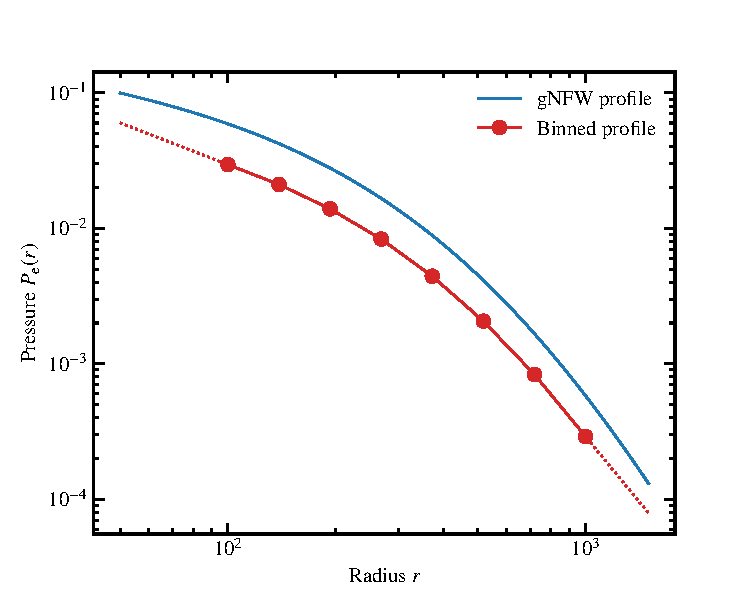
\includegraphics[width=.65\linewidth]{Figures/Chap_panco/gnfw_np.pdf}
    \label{fig:panco:gnfw_np}
\end{SCfigure*}

% ------------------------------------------------------------------------------------ %
\subsection{Modèle de carte de brillance de surface SZ}

Le profil de pression considéré est ensuite intégré le long de la ligne de visée afin d'obtenir une carte de paramètre de Compton $y$ dans la région de l'amas.
Dans le cas d'un modèle gNFW, l'intégrale de l'équation (\ref{eq:panco:y_los}) n'a pas de solution analytique, et une intégration numérique est utilisée, en considérant un grand nombre de pas espacés logarithmiquement le long de la ligne de visée afin de limiter les artefacts d'intégration.
Dans le cas d'un modèle non-paramétrique, l'intégrale de l'équation (\ref{eq:panco:y_abel}) est la somme des intégrales analytiques du profil de pression dans chacune des coquilles sphériques \cite{romero_multi-instrument_2018}.

La carte de paramètre de Compton obtenue doit ensuite être convertie en unités de brillance de surface afin d'être comparable aux données observées.
Le facteur de conversion dépend des bandes passantes effectives de NIKA2 (et donc des conditions atmosphériques au moment des observations), mais également du lobe de l'instrument.
Il dépend également de la forme du spectre de l'effet SZ, et donc de la température du milieu intra-amas du fait des corrections relativistes à l'effet SZ, comme décrit en section~\mypageref{sec:sz}.
En pratique, \texttt{PANCO2} traite ce facteur de conversion comme un paramètre de nuisance de l'analyse, ce qui permet de tenir compte de l'incertitude systématique liée à la variabilité de ce coefficient due aux conditions d'observations.

Les cartes de l'effet SZ réalisées par NIKA2 sont affectées par deux formes de filtrage.
Tout d'abord, l'image du ciel est convoluée par le lobe instrumental caractéristique du couplage entre NIKA2 et le télescope (décrit au chapitre~\ref{chap:nika2}).
Le modèle de carte de brillance de surface SZ est donc convolué par un filtre gaussien de largeur à mi-hauteur spécifiée par l'utilisateur.
Les cartes sont également affectées par le filtrage découlant de la procédure de soustraction du bruit des données en temps de NIKA2.
Ce filtrage est estimé par le calcul de la fonction de transfert présenté au chapitre \ref{chap:decorr}, et la carte de modèle est également convoluée par cette fonction de transfert.
La carte résultante est donc une carte étalonnée en unités de brillance de surface, affectée par le lissage des petites échelles angulaires caractéristique du couplage entre NIKA2 et le télescope, et par le filtrage des grandes échelles provenant de l'analyse des données brutes.
Elle peut donc être comparée à la carte de brillance de surface de l'effet SZ observée par NIKA2.

% ------------------------------------------------------------------------------------ %
\subsection{Contamination par des sources ponctuelles}\label{sec:panco_ps}

Le signal astrophysique mesuré par NIKA2 lors des observations d'amas de galaxies est la somme des contributions des différents objets présents le long de la ligne de visée.
Les contributeurs majeurs sont le milieu intra-amas par effet SZ, constituant l'observable d'intérêt pour les études présentées dans cette thèse ; ainsi que l'émission de sources ponctuelles.
Cette émission, par nature positive, peut compenser partiellement ou totalement le décrément SZ détecté dans les cartes NIKA2 à 150 GHz, et peut donc induire un biais négatif dans le profil de pression du milieu intra-amas reconstruit à partir des observations NIKA2.
La contamination résultante doit donc être prise en compte dans les mesures de propriétés du milieu intra-amas afin de ne pas souffrir de ce biais lors de l'utilisation des résultats du grand programme SZ en cosmologie.

Cette contamination peut être prise en compte en soustrayant des modèles de sources des données NIKA2.
Pour cela, il est nécessaire de connaitre la valeur du flux de chaque source, et une mauvaise estimation de ces flux peut induire une erreur dans les propriétés thermodynamiques mesurées.
\texttt{PANCO2} offre la possibilité de traiter cette contamination comme un paramètre de nuisance dans l'ajustement du profil de pression du milieu intra-amas.
Cette approche, présentée plus en détail dans le chapitre \ref{chap:actj0215}, permet de propager l'incertitude sur les flux des différentes sources ponctuelles à la mesure des propriétés thermodynamiques du milieu intra-amas.
Pour cela, des sources modélisées comme le lobe de NIKA2\footnote{Voir section~\ref{sec:nk_perf}.} peuvent être ajoutées au modèle de carte de brillance de surface présenté précédemment avant que celle-ci ne soit comparée aux données.
Les flux de ces sources sont alors considérés comme des paramètres supplémentaires du modèle.
La distribution de probabilité du flux de chaque source, obtenue avec \texttt{PSTools} (voir section \ref{sec:decor:pstools}), peut alors être utilisée comme \prior\ sur le paramètre, comme nous le verrons en section \ref{sec:panco:priors}.

% ------------------------------------------------------------------------------------ %
\subsection{Signal SZ intégré}

La couverture angulaire des observations SZ réalisées par NIKA2 est limitée par le filtrage des grandes échelles angulaires issu de la soustraction du bruit atmosphérique.
Ce filtrage se caractérise par une perte de signal en périphérie de l'amas, ce qui empêche l'établissement de contraintes fortes sur le profil de pression du milieu intra-amas dans ces régions.
Une information sur ce signal est contenue dans le signal SZ intégré de l'amas, mesuré dans les relevés à plus grand champ de vue desquels est issu le catalogue du grand programme SZ, à savoir les relevés \textit{Planck} \cite{planck_collaboration_planck_2016-3} et ACT \cite{hasselfield_atacama_2013}.
Ce signal est proportionnel à l'intégrale sphérique du profil de pression considéré jusqu'à un rayon donné $R$:
\begin{equation}
    Y_R = 4 \pi \frac{\sigma_\textsc{t}}{m_\e c^2} \int_0^R r^2 P_\e(r) \d r.
\end{equation}
Cette valeur peut donc être calculée à partir du modèle de profil de pression considéré, et comparée aux valeurs reportées dans les relevés SZ, imposant une contrainte effective sur le profil de pression dans les régions non contraintes par les observations NIKA2.
Les valeurs de $Y_{500}$ sont disponibles pour tous les amas du grand programme SZ de NIKA2, mesurées par \textit{Planck} ou ACT, et sont systématiquement utilisées afin d'améliorer la contrainte du profil de pression dans la périphérie de l'amas.

% ==================================================================================== %
\section{Ajustement par méthode Monte Carlo à Chaînes de Markov}
\label{sec:panco:fit}

Afin de déterminer le profil de pression du milieu intra-amas, le modèle de carte de brillance de surface décrit dans la section précédente est ajusté sur les données NIKA2 en utilisant un algorithme Monte Carlo à Chaînes de Markov (MCMC).
L'objectif est donc de trouver la distribution de probabilités des paramètres étant données les mesures effectuées par NIKA2.
Cette distribution, dite postérieure, est donnée par le théorème de Bayes :
\begin{equation}
    \label{eq:panco:bayes}
    P(\vartheta \,|\, D) = \frac{P(D \,|\, \vartheta) \, P(\vartheta)}{P(D)},
\end{equation}
où $\vartheta$ est le vecteur formé par les différents paramètres de l'analyse, résumés dans le tableau \ref{tab:panco:params}, et $D$ représente les données mesurées, qui dans le cas de \texttt{PANCO2}, sont la carte de brillance de surface mesurée par NIKA2 et le signal SZ intégré mesuré par ACT ou \textit{Planck}. \\
La distribution $P(D \,|\, \vartheta)$ est la fonction de vraisemblance comparant le modèle aux données, et $P(\vartheta)$ est notre connaissance \prior\ sur les valeurs des paramètres de l'analyse.
$P(D)$ est traitée comme une constante de normalisation permettant à l'équation (\ref{eq:panco:bayes}) d'être intégrable à 1.

% ------------------------------------------------------------------------------------ %
\subsection{Fonction de vraisemblance} \label{sec:panco:likelihood}

La fonction de vraisemblance, ou \textit{likelihood} en anglais, est la probabilité qu'un jeu de données $D$ soit issu d'un modèle $\vartheta$.
Dans \texttt{PANCO2}, j'ai choisi d'utiliser une fonction de vraisemblance Gaussienne multivariée dont chacun des pixels de la carte NIKA2 est une dimension :
\begin{equation}
    \label{eq:panco:like}
    \mathrm{log} \, P(D \, | \, \vartheta)
    = - \frac{1}{2}
        \big(D_\textsc{n} - \mathcal{M}_\textsc{n}(\vartheta)\big)^{\rm T}
        \Sigma_\textsc{n}^{-1}
        \big(D_\textsc{n} - \mathcal{M}_\textsc{n}(\vartheta)\big)
      - \frac{1}{2}
        \left(\frac{Y_R^{\rm meas.} - Y_R(\vartheta)}{\Delta Y_R^{\rm meas.}}\right)^2
      - \Delta_{\rm mass},
\end{equation}
où $D_\textsc{n}$ représente la carte NIKA2 à 150 GHz, $\mathcal{M}_\textsc{n}(\vartheta)$ le modèle de carte calculé à partir des paramètres $\vartheta$, et $\Sigma_\textsc{n}$ la matrice de covariance du bruit ;
$Y_R^{\rm meas.}$ et $\Delta Y_R^{\rm meas.}$ sont la mesure de signal SZ intégré dans un rayon $R$ et son incertitude, et $Y_R(\vartheta)$ le signal SZ intégré correspondant au modèle considéré (dans la suite, nous utiliserons $R = R_{500}$). \\
Cette fonction de vraisemblance permet donc de comparer un modèle aux observations réalisées avec NIKA2, en tenant également compte de la contrainte sur le paramètre de Compton intégré mesuré par \textit{Planck} ou ACT.
Dans le cadre d'un modèle gNFW, et si des données X sont fournies par l'utilisateur, le terme $\Delta_{\rm mass}$ est ajouté afin d'interdire les points pour lesquels le profil de masse décroit avec le rayon:
\begin{equation}
    \Delta_{\rm mass} =
        \begin{cases}
            \; 0 \;\text{si}\; \mathrm{d}M^{\rm HSE} / \mathrm{d}r \geqslant 0 \,\forall r, \\
            \; -\infty \;\text{sinon,}
        \end{cases}
\end{equation}
où $M^{\rm HSE}$ est calculé à partir de l'équation de l'équilibre hydrostatique (\ref{eq:mhse}). \\
Ce terme permet de restreindre l'espace des paramètres aux profils de pression ayant un sens physique, la masse contenue dans un rayon croissant ne pouvant pas diminuer.
Il n'est toutefois pas implémenté lors de l'ajustement d'un modèle non-paramétrique.
En effet, de telles analyses peuvent avoir pour objectif la mesure de surpressions locales, par exemple dues à des chocs.
Dans ces cas où l'équilibre hydrostatique n'est pas respecté, l'imposition d'une telle contrainte empêcherait la détection de telles particularités du profil de pression.
Cette contrainte n'est par conséquent imposée qu'au cours de l'ajustement de modèles gNFW, pour lesquels des fluctuations de pression ne sont de toute façon pas détectables, et qui bénéficient de la réduction de l'espace des paramètres au vu des fortes corrélations entre ces derniers.

% ------------------------------------------------------------------------------------ %
\subsection{Distribution \prior\ des paramètres}
\label{sec:panco:priors}

L'approche bayésienne utilisée dans \texttt{PANCO2} requiert la définition d'une distribution de probabilité \prior\ des paramètres $\vartheta$ qui sera combinée à la fonction de vraisemblance pour préciser la connaissance des paramètres.
Cette distribution est modélisée comme le produit de distributions définies individuellement pour chaque paramètre, soit en considérant chaque paramètre comme indépendant.
\texttt{PANCO2} propose plusieurs possibilités de distribution \prior\ pour chaque paramètre, résumées dans le tableau \ref{tab:panco:params}.
Notons en particulier que les paramètres correspondant au flux des sources ponctuelles peuvent prendre comme \prior\ la distribution de probabilité issue de \texttt{PSTools}, obtenue par ajustement du spectre des sources (voir section \ref{sec:decor:pstools}).

\afterpage{
\begin{table}[t]
    \setlength{\tabcolsep}{15pt}
    \small
    \centering
    \begin{tabular}{c l l}
        \toprule
        Paramètre & Description & Distribution \prior \\
        \midrule
        \midrule
        \multicolumn{3}{c}{\itshape Paramètres d'intérêt pour un modèle gNFW} \\
        \midrule
        $P_0, r_{\rm p}, a, b, c$ & Paramètres du profil de pression & -- Gaussiennes définies par l'utilisateur \\
          & & -- Uniformes avec limites choisies par l'utilisateur \\
        \midrule
        \multicolumn{3}{c}{\itshape Paramètres d'intérêt pour un modèle non-paramétrique} \\
        \midrule
        $P_i, \; i = 0 \dotsc n_{\rm bins}$ & Valeurs de pression & Uniformes entre 0 et 1 ${\rm keV \cdot cm^{-3}}$ \\
        \midrule
        \multicolumn{3}{c}{\itshape Paramètres de nuisance} \\
        \midrule
        $C_{\rm conv}$ & Conversion de $y$ en Jy/beam & Gaussienne définie par l'utilisateur \\[3pt]
        $Z$ & Niveau zéro de la carte & Gaussienne $\N(0,0.1 \; {\rm mJy/beam})$ \\[3pt]
        $F_i, \; i = 0 \dotsc n_{\rm PS}$ & Flux des sources ponctuelles & -- Distribution issue de \texttt{PSTools} (section \ref{sec:decor:pstools}) \\
        & & -- Uniformes avec limites définies par l'utilisateur \\
        \bottomrule
    \end{tabular}
    \caption{%
        Liste des paramètres utilisés par \texttt{PANCO2} pour modéliser les cartes SZ construites à partir d'observations NIKA2.
        La dernière colonne indique les distributions \prior\ utilisables pour chaque paramètre.
    }
    \label{tab:panco:params}
\end{table}
}

% ------------------------------------------------------------------------------------ %
\subsection{Échantillonnage de la distribution de probabilités}
\label{sec:mcmc_sampling}

L'ajustement du profil de pression est réalisé par échantillonnage Monte Carlo à Chaînes de Markov (MCMC) de la distribution postérieure définie par l'équation (\ref{eq:panco:bayes}).
L'avantage du MCMC par rapport à une maximisation de fonction de vraisemblance est l'obtention d'un ensemble de points de l'espace des paramètres distribués selon la postérieure de notre analyse, qui pourra ensuite être transposé dans l'espace des propriétés physiques du milieu intra-amas.

\subsubsection{Principe du MCMC} % --------------------------------------------------- %
Le principe de fonctionnement du MCMC repose sur une exploration de l'espace des paramètres par marche aléatoire, conditionnée par la valeur de la distribution de probabilités aux points visités.
Cette marche aléatoire peut être décrite par une série d'étapes successives :

\begin{enumerate}[leftmargin=*]
    \item La marche aléatoire commence en un point de l'espace des paramètres de coordonnées définies par un vecteur $\vartheta$.
        La valeur de la distribution de probabilités considérée est $P(\vartheta)$.
    \item Une position proche dans l'espace des paramètres, $\vartheta'$, est tirée au hasard d'après une fonction de proposition prédéfinie.
    \item Si $P(\vartheta') \geqslant P(\vartheta)$, alors $\vartheta'$ est automatiquement acceptée comme nouvelle position de l'échantillonneur ; sinon, elle est aléatoirement acceptée ou non avec une probabilité d'autant plus faible que $P(\vartheta') < P(\vartheta)$, nommée probabilité d'acceptance.
    \item La procédure est répétée autant de fois que nécessaire pour obtenir un nombre d'échantillons jugé suffisant.
\end{enumerate}

Ce processus peut être réalisé en parallèle par plusieurs marcheurs, créant chacun simultanément un ensemble de points nommé chaîne de Markov.
L'ensemble des positions $\vartheta$ acceptées par l'échantillonneur est alors distribué selon la fonction de distribution de probabilités considérée.

%\subsubsection{Échantillonneur utilisé dans \texttt{PANCO2}}
Un exemple commun de MCMC est donné par l'algorithme de Metropolis-Hastings \cite{metropolis_monte_1949,hastings_monte_1970}, où la fonction de proposition est une distribution Gaussienne de largeur constante et la probabilité d'acceptance est donnée par $p = P(\vartheta') < P(\vartheta)$.
Celui-ci est limité par la nécessité de définir au préalable une fonction de proposition immuable au cours de l'échantillonnage.
\texttt{PANCO2} utilise la librairie \texttt{emcee} \cite{foreman-mackey_emcee_2019}, proposant plusieurs implémentations en Python d'échantillonneurs adaptant leur fonction de proposition au cours de l'échantillonnage, introduits par \myciteauthor{goodman_ensemble_2010}.
En particulier, dans le cas de \texttt{PANCO2}, l'échantillonneur retenu est celui offrant les meilleures performances en termes d'échantillons indépendants générés par unité de temps, l'échantillonneur \texttt{DEMove} \cite{nelson_run_2013}.

\begin{figure}[t]
    \centering
    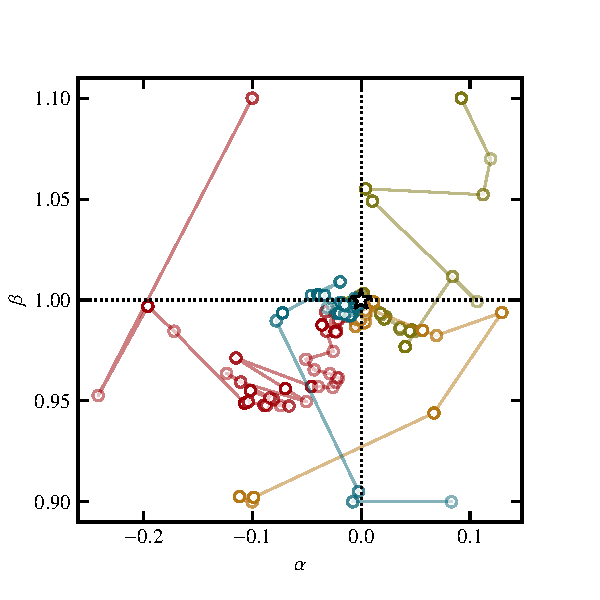
\includegraphics[width=.495\textwidth]{Figures/Chap_panco/mcmc_params.pdf}
    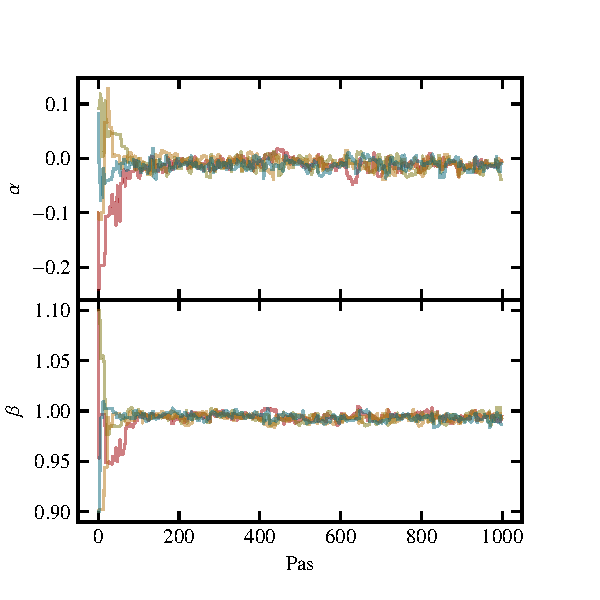
\includegraphics[width=.495\textwidth]{Figures/Chap_panco/mcmc_trace.pdf}
    \caption{
        Illustration du mouvement des chaînes d'un échantillonneur MCMC dans le cas d'une régression à deux paramètres $(\alpha, \beta)$, dans l'espace des paramètres (\textit{gauche}) et projeté pour chacun des paramètres individuellement (\textit{droite}).
        Chaque couleur représente une chaîne de Markov.
        L'étoile dans le panneau gauche représente le maximum de la distribution postérieure considérée.
    }
    \label{fig:panco:mcmc}
\end{figure}

\subsubsection{Convergence des chaînes et autocorrélation} % ------------------------- %
L'échantillonnage MCMC réalisé par \texttt{PANCO2} est automatiquement stoppé lorsque la convergence des chaînes a été atteinte, c'est-à-dire à partir de l'instant où l'ajout de nouveaux points aux chaînes de Markov n'apporterait pas d'information significative par rapport à ceux déjà générés.
La convergence est basée sur trois critères : l'adaptation des chaînes, leur mélange, et leur autocorrélation, décrite ci-après.

Le point de départ du MCMC dans l'espace des paramètres est arbitraire et ne se trouve pas nécessairement dans la région d'intérêt.
Par conséquent, il est nécessaire d'amputer chaque chaîne d'une longueur d'adaptation, correspondant au nombre de pas nécessaires à chaque marcheur pour rejoindre cette région d'intérêt.
Cette longueur, qualifiée de \textit{burn-in}, est systématiquement ignorée afin de ne considérer que les échantillons correspondant à des chaînes stationnaires et ne dépendant pas du point de départ arbitraire.
La figure \ref{fig:panco:mcmc} illustre cette adaptation : le panneau gauche montre le déplacement des marcheurs vers la région d'intérêt, symbolisée par l'étoile noire, et le panneau droit permet d'estimer une longueur de \textit{burn-in} d'environ une centaine de pas.

Le mélange des chaînes quantifie la similarité entre les distributions de points générés par chacune d'entre elles.
Des chaînes mélangées seront donc stationnaires et statistiquement similaires, comme illustré dans le panneau droit de la figure \ref{fig:panco:mcmc} dans le régime stationnaire.
Un critère permettant d'évaluer ce mélange est le critère de \myciteauthor{gelman_inference_1992}:
\begin{equation}
    \label{eq:panco:rhat}
    \hat{R} \equiv \sqrt{\frac{V}{W}} < 1.02
\end{equation}
où $W$ est la variance moyenne des échantillons d'une chaîne et $V$ la variance entre les différentes chaînes.

Les échantillons produits par la marche aléatoire décrite ci-dessus ne sont pas indépendants.
En effet, la position de chaque point dépend par construction de la position précédente.
On parle alors d'autocorrélation des chaînes.
La longueur moyenne séparant deux points pouvant être considérés indépendants peut être calculée d'après la série de positions acceptées formant la chaîne de Markov:
\begin{equation}
    \tau = 1 + 2 \sum_{i=1}^{n} \rho(\vartheta_0, \vartheta_i)
\end{equation}
où $n$ est la longueur de la chaîne considérée, et $\rho(\vartheta_0, \vartheta_i)$ est le coefficient de corrélation entre $\vartheta_0$ et $\vartheta_i$.

À intervalle régulier au cours de l'échantillonnage, \texttt{PANCO2} évalue ces trois critères, et accepte la convergence si :
\begin{itemize}[leftmargin=*]
    \setlength\itemsep{5pt}
    \item Toutes les chaînes ont parcouru une longueur supérieure à cinq fois la longueur de \textit{burn-in} définie par l'utilisateur ;
    \item Plus des deux tiers des chaînes passent le test de \citeauthor{gelman_inference_1992} (\ref{eq:panco:rhat}) ;
    \item Ces chaînes ont parcouru plus de cinquante fois leur longueur d'autocorrélation.
\end{itemize}
Les valeurs numériques utilisées dans ces tests sont des paramètres de l'analyse pouvant être modifiés par l'utilisateur.
Le choix particulier de deux tiers des chaînes et cinquante longueurs d'autocorrélation, utilisé par défaut, provient des tests sur simulations développés en section \ref{sec:panco:simus}.

% ------------------------------------------------------------------------------------- %
\subsection{Évaluation des propriétés thermodynamiques} \label{sec:panco:thermo}

Les chaînes de Markov produites par l'échantillonneur constituent un ensemble de points suivant la distribution de probabilité postérieure dans l'espace des paramètres du modèle.
On peut les écrire comme un vecteur $\mathbf{\vartheta}$, de dimension $n$ le nombre de points dans les chaînes, dont chaque composante $i \in [1 \dots n]$ est un vecteur dans l'espace des paramètres.
Cela permet de définir un vecteur de profils de pression $\mathbf{P}(r)$, dont chaque composante $i$ est le profil associé aux paramètres du point $\mathbf{\vartheta}_i$ des chaînes de Markov:
\begin{equation}
    \label{eq:panco:press_vec}
    \mathbf{P}(r) = P_\e(r, \mathbf{\vartheta_i}),
\end{equation}
où $P_\e(r)$ est le modèle de profil de pression choisi, gNFW ou non-paramétrique. \\
La distribution des composantes de $\mathbf{P}(r)$ permet donc d'étudier la distribution postérieure dans l'espace non plus des paramètres, mais des profils de pression.
On peut ainsi calculer l'incertitude sur le profil de pression comme la dispersion des composantes de $\mathbf{P}(r)$, ou encore comme les quantiles de cette distribution (les deux options sont implémentées dans \texttt{PANCO2}, et peuvent être choisis par l'utilisateur).

\subsubsection{Interpolations du modèle non-paramétrique} % --------------------------- %
\label{sec:panco:interp_np}
Dans le cas d'un modèle non-paramétrique, les paramètres du modèle sont les valeurs du profil de pression à différents rayons choisis par l'utilisateur.
La mesure de la pression à un rayon $r$ quelconque nécessite donc une interpolation (ou l'extrapolation) à partir de ces points.
\texttt{PANCO2} propose trois méthodes différentes, à choisir par l'utilisateur, pour interpoler le profil de pression pour la présentation des résultats finaux:
\begin{itemize}[leftmargin=*]
    \setlength\itemsep{0pt}
    \item L'interpolation en loi de puissance des points.
        C'est la méthode utilisée au cours de l'ajustement (voir équation \ref{eq:panco:nonparam}), et donc la plus naturelle.
        Cependant, comme nous l'avons décrit en \mypageref{sec:panco:p_prof}, le modèle non-paramétrique est une fonction dont la dérivée n'est pas continue.
        Le profil de masse hydrostatique étant justement proportionnel à cette dérivée, il peut présenter des discontinuités, rendant difficile l'estimation d'un profil de masse à partir de l'ajustement d'un tel modèle.
    \item Une interpolation en \textit{splines} du profil de pression.
        Si cette option est choisie, chacune des composantes du vecteur $\mathbf{P}(r)$ est interpolée par une fonction \textit{spline} dans le plan log-log, résultant en un profil de pression lisse et de dérivée continue.
        Cette méthode présente l'avantage de réaliser un lissage du profil, permettant l'estimation d'un profil de masse continu, tout en gardant l'aspect non-paramétrique du modèle utilisé pour l'ajustement.
        Cependant, son extrapolation est risquée, car les splines ne disposent d'aucune contrainte au delà de la région couverte par les rayons $R$ considérés dans le modèle.
    \item Une interpolation par un modèle gNFW.
        Dans ce cas, un modèle gNFW est ajusté sur chacune des composantes de $\mathbf{P}(r)$, et le modèle ajustant le mieux chaque profil est utilisé comme fonction d'interpolation.
        Les profils obtenus sont lisses et de dérivées continues, et leur extrapolation est rendue possible par le peu de variété dans les formes que peut prendre le modèle gNFW.
        En revanche, l'identification d'écarts à ce modèle n'est plus possible.
\end{itemize}
Quelle que soit la méthode choisie, elle permet de calculer le vecteur $\mathbf{P}(r)$ pour toute valeur de $r$ choisie.
La distribution des composantes du vecteur peut alors être étudiée pour évaluer l'incertitude sur le profil de pression.
La différence entre les profils de pression et de masse hydrostatique obtenus par l'utilisation de ces trois méthodes sera détaillée dans la section suivante (page \pageref{sec:panco:interp_np_results}), et illustrée en figure \ref{fig:panco:interp_np}.

\subsubsection{Profils thermodynamiques par combinaison avec les mesures X} % --------- %
\label{sec:panco:thermo_profiles_x}
Une fois que le vecteur $\mathbf{P}(r)$ a été construit, en calculant un profil de pression pour chaque jeu de paramètres issu des chaînes de Markov, celui-ci est combiné aux mesures X pour caractériser plus en détail les propriétés thermodynamiques du milieu intra-amas.
Pour cela, le vecteur $\mathbf{P}(r)$ est combiné avec le profil de densité X pour obtenir un vecteur de profils de température $\mathbf{T}$  d'après l'équation (\ref{eq:temperature}):
\begin{equation}
    k_\textsc{b} \mathbf{T}(r) = \mathbf{P}(r) \,\big/\, n_\e(r)
\end{equation}
et d'entropie $\mathbf{K}$ d'après l'équation (\ref{eq:entropy}):
\begin{equation}
    \mathbf{K}(r) = \mathbf{P}(r)\;n_\e^{-5/3}(r),
\end{equation}
et un vecteur de profils de masse à partir de l'équation de l'équilibre hydrostatique (\ref{eq:mhse}).
Comme pour le profil de pression, la dispersion des composantes de ces vecteurs donne l'incertitude sur les profils.
Comme nous l'avons vu en \mypageref{sec:lpsz_sci}, ces quantités permettent l'étude de la structure de l'amas et de son état dynamique, en exploitant la synergie entre observations SZ à haute résolution et X.
Une fois mesurées pour tout l'échantillon, elles pourront mener à des travaux sur le lien entre la physique de ces objets et les incertitude systématiques liées à leur exploitation cosmologique.

\subsubsection{Grandeurs caractéristiques intégrées} % -------------------------------- %
\label{sec:panco:integrated_qties}
Dans le cas du grand programme SZ de NIKA2, l'objectif est la mesure du profil de pression des amas, mais également de la relation d'échelle liant le paramètre de Compton $Y_{500}$ intégré dans un rayon $R_{500}$ à la masse $M_{500}$ contenue dans ce même rayon.
\texttt{PANCO2} permet de mesurer ces grandeurs en calculant le profil de masse hydrostatique à partir de l'équation de l'équilibre hydrostatique (\ref{eq:mhse}), puis en en déduisant le profil de contraste de densité $\delta_c(r)$ :
\begin{equation}
    \label{eq:panco:delta_c}
    \delta_c(r) = \frac{M_\mathrm{HSE}(<r)}{\rho_c(z) \times \frac{4}{3} \pi r^3}.
\end{equation}
où $\rho_c(z)$ est la densité critique de l'Univers au redshift $z$ de l'amas. \\
La procédure utilisée pour calculer les grandeurs intégrées est la suivante:
\begin{enumerate}[leftmargin=*]
    \item Le vecteur de profils de masse hydrostatique $\mathbf{M}_{\rm HSE}(r)$ est utilisé pour calculer un vecteur de profils de contraste de densité par l'équation (\ref{eq:panco:delta_c});
    \item Une valeur de $R_{500,i}$ est calculée pour chacune des composantes $i$ du vecteur de profils de contraste, en trouvant le rayon pour lequel il est égal à $500$;
    \item Une valeur de $Y_{500, i}$ est calculée pour chacune des composantes $i$ du vecteur $\mathbf{P}(r)$ par:
    \begin{equation}
        Y_{500, i} = 4\pi \frac{\sigma_\textsc{t}}{m_\e c^2}\int^{R_{500, i}} r^2 P_i(r) \, \d r,
    \end{equation}
    et une valeur de $M_{500, i}$ à partir des profils de masse hydrostatique:
    \begin{equation}
        M_{500, i} = M_i(R_{500, i}).
    \end{equation}
\end{enumerate}
Le résultat de cette procédure est donc un vecteur pour chacune des grandeurs caractéristiques $R_{500}$, $Y_{500}$ et $M_{500}$, dont chaque composante $i$ correspond à la grandeur estimée pour le point $\mathbf{\vartheta}_i$ des chaînes de Markov.
La distribution des composantes représente alors la distribution postérieure échantillonnée par le MCMC, dans l'espace des grandeurs intégrées, et peut être utilisée pour calculer les incertitudes entre les paramètres.
On note que les grandeurs intégrées sont par construction corrélées, comme déjà mentionné au chapitre \ref{chap:amas}.
Cette méthode d'estimation des grandeurs intégrées permet la mesure de cette corrélation en calculant la covariance des grandeurs intégrées mesurées pour chaque échantillon des chaînes de Markov.
La connaissance de cette covariance est cruciale à l'estimation des relations d'échelle, comme nous le verrons au chapitre \ref{chap:scaling}.
Les produits de \texttt{PANCO2} pourront donc être utilisés directement pour la mesure de la relation d'échelle $Y_{500}-M_{500}$ par la collaboration NIKA2.

% ===================================================================================== %
\section{Validation de \texttt{PANCO2} sur des amas simulés}
\label{sec:panco:simus}

Afin de s'assurer de la capacité de \texttt{PANCO2} à produire des mesures correctes de profil de pression, il est nécessaire de le tester sur des cartes d'amas dont le profil de pression est connu, et ainsi de comparer le profil évalué avec la vérité.
Pour cela, il est possible soit d'utiliser des observations réelles d'amas connus au profil de pression déjà caractérisé par d'autres instruments, soit de s'appuyer sur des simulations.
La première approche présente l'avantage de faire appel à des données réelles, mais est limitée par la connaissance imparfaite de l'amas observé.
L'analyse de simulations permet de connaitre parfaitement les propriétés physiques d'entrée, mais est limitée par la nécessité de créer des données réalistes et représentatives d'observations réelles.
La validation de \texttt{PANCO2} emploie la seconde approche, utilisant des amas synthétiques analytiques, puis un échantillon d'amas issu de la simulation hydrodynamique MUSIC \cite{sembolini_music_2013}.

% ------------------------------------------------------------------------------------- %
\subsection{Simulations d'amas simples} \label{sec:panco:demo}

La première analyse de validation de \texttt{PANCO2} est réalisée sur une carte d'amas synthétique similaire à l'un des amas du LPSZ.
Nous avons choisi l'amas \act, un des amas de faible masse et haut redshift de l'échantillon, dont les observations réelles seront présentées et analysées au chapitre \ref{chap:actj0215}.

Le milieu intra-amas de cette source synthétique est modélisé par un profil de pression gNFW, correspondant à celui mesuré par l'analyse effectuée sur les observations NIKA2 de l'amas \cite{keruzore_exploiting_2020}.
Des cartes de l'amas sont ensuite produites en intégrant ce profil de pression le long de la ligne de visée, et en filtrant la carte obtenue par le lobe de NIKA2 et par la fonction de transfert réelle de l'analyse.
Enfin, une réalisation de bruit blanc correspondant au niveau de bruit résiduel dans la carte de \act\ est ajoutée à la carte.

Les cartes obtenues sont ajustées avec \texttt{PANCO2} afin de tester sa validité sur des cas simples d'amas sphériques idéaux.
Cette analyse utilise un profil de pression non-paramétrique, dont les valeurs de rayons $R$ sont définies pour couvrir le signal attendu avec NIKA2, de son lobe à son champ de vue.
Cette distribution de rayons sera détaillée en \mypageref{sec:panco:binning}.
Dans cette section, nous décrivons les résultats pour cet amas synthétique, et présentons par la même occasion les figures produites par \texttt{PANCO2}.
Notons qu'une analyse similaire a été menée pour l'ajustement d'un modèle gNFW.
Les résultats sont très similaires pour les deux modèles (offrant une reconstruction non-biaisée du profil de pression), aussi ne présentons-nous ici que les résultats de l'ajustement d'un modèle non-paramétrique.

\subsubsection{Résultats de l'ajustement} % ------------------------------------------- %
Les résultats de l'ajustement permettent d'observer un accord entre le modèle ajusté par \texttt{PANCO2} et la vérité, utilisée pour générer les cartes.
La figure \ref{fig:panco2:actlike_dmr} montre la carte d'entrée et le meilleur ajustement de cette carte obtenu par \texttt{PANCO2}.
La différence entre ces deux cartes, représentant les résidus de l'ajustement, est compatible avec du bruit et ne permet pas d'identifier d'écart entre la vérité et l'ajustement.

\begin{figure*}[t]
    \centering
    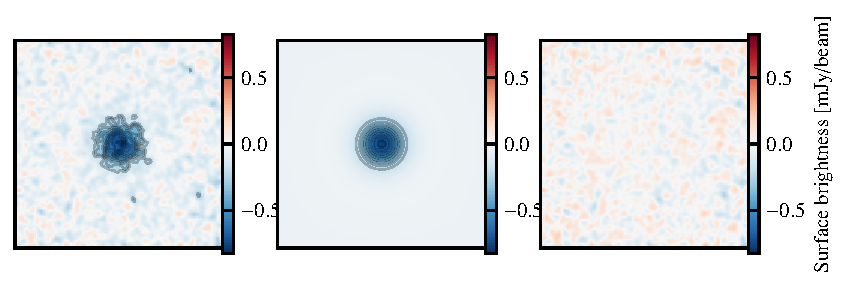
\includegraphics[width=\linewidth]{Figures/Chap_panco/demo_plots/data_model_residuals.pdf}
    \caption{
        Carte simulée de \act\ (\textit{gauche}), carte de modèle ajustée par \texttt{PANCO2} (\textit{centre}), et différence entre les deux cartes (\textit{droite}).
        La région représentée est la même pour les trois cartes, et représente un carré de 5' de côté centré sur le centre simulé de l'amas.
        Les contours gris sont les niveaux de signal-sur-bruit, commençant à $3\sigma$ et espacés de $1\sigma$.
    }
    \label{fig:panco2:actlike_dmr}
\end{figure*}

\subsubsection{Chaînes de Markov et distribution postérieure des paramètres} % -------- %
La figure \ref{fig:panco2:actlike_chains} montre les chaînes de Markov, à savoir l'évolution des positions acceptées des marcheurs dans l'espace des paramètres avec le temps.
Chaque couleur correspond à un marcheur.
On voit que les chaînes ont atteint un état stationnaire, où elles n'évoluent plus à grande échelle et oscillent autour d'une valeur de paramètre correspondant à la valeur maximisant la distribution postérieure.
On voit également l'évolution à partir du point de départ, au cours des $\sim 200$ premiers pas.
La longueur de \textit{burn-in} retirée, représentée en gris, est de 1000 pas.

\begin{figure*}[t]
    \centering
    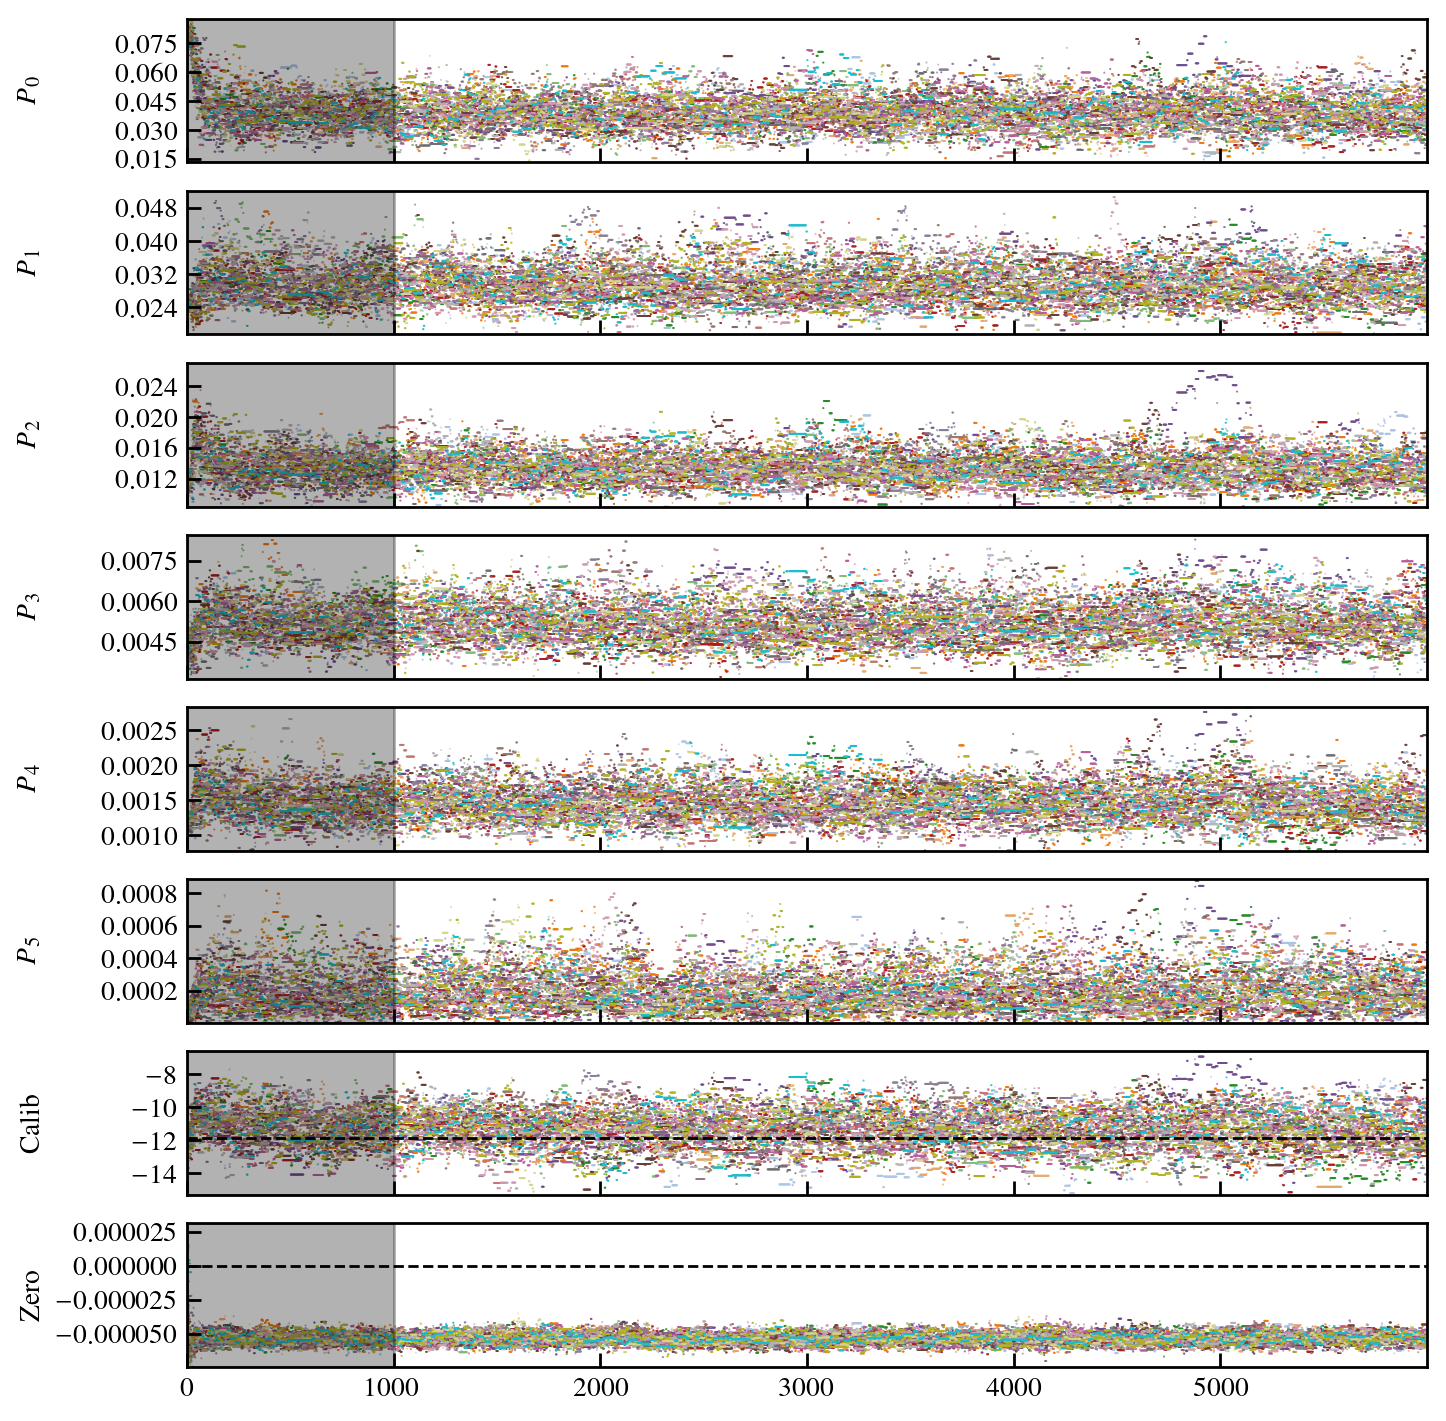
\includegraphics[width=0.9\textwidth]{Figures/Chap_panco/demo_plots/chains.png}
    \caption{
        Évolution des chaînes de Markov dans l'espace des paramètres avec le nombre de pas.
        Chaque couleur représente une chaîne distincte.
        La région grise correspond au \textit{burn-in} retiré pour l'analyse.
        Les lignes noires pointillées correspondent au vraies valeurs du coefficient de conversion et du niveau zéro de la carte.
    }
    \label{fig:panco2:actlike_chains}
\end{figure*}

La figure \ref{fig:panco2:actlike_corner} montre la distribution des positions des chaînes de Markov, c'est-à-dire la distribution postérieure, marginalisée sur chacun des paramètres (diagonale) et sur chaque combinaison de deux paramètres (éléments extra-diagonaux).
Cette figure représente donc la distribution postérieure échantillonnée dans l'espace des paramètres, qui sont les paramètres du profil de pression $P_i$, le coefficient de conversion et le niveau zéro de la carte.
Cette figure illustre donc à la fois les distributions de probabilité des paramètres et les corrélations entre ces paramètres.
On voit par exemple une forte corrélation entre le dernier point en pression $P_5$ et le niveau zéro de la carte: en effet, ajouter de la pression à très grand rayon, du fait de l'intégration le long de la ligne de visée, revient à ajouter un plateau quasi-constant à la carte.
La distribution de $\chi^2$ par degrés de liberté est également représentée, et est centrée en une valeur proche de 1, indiquant un bon ajustement des données par le modèle.

\begin{figure*}[p]
    \centering
    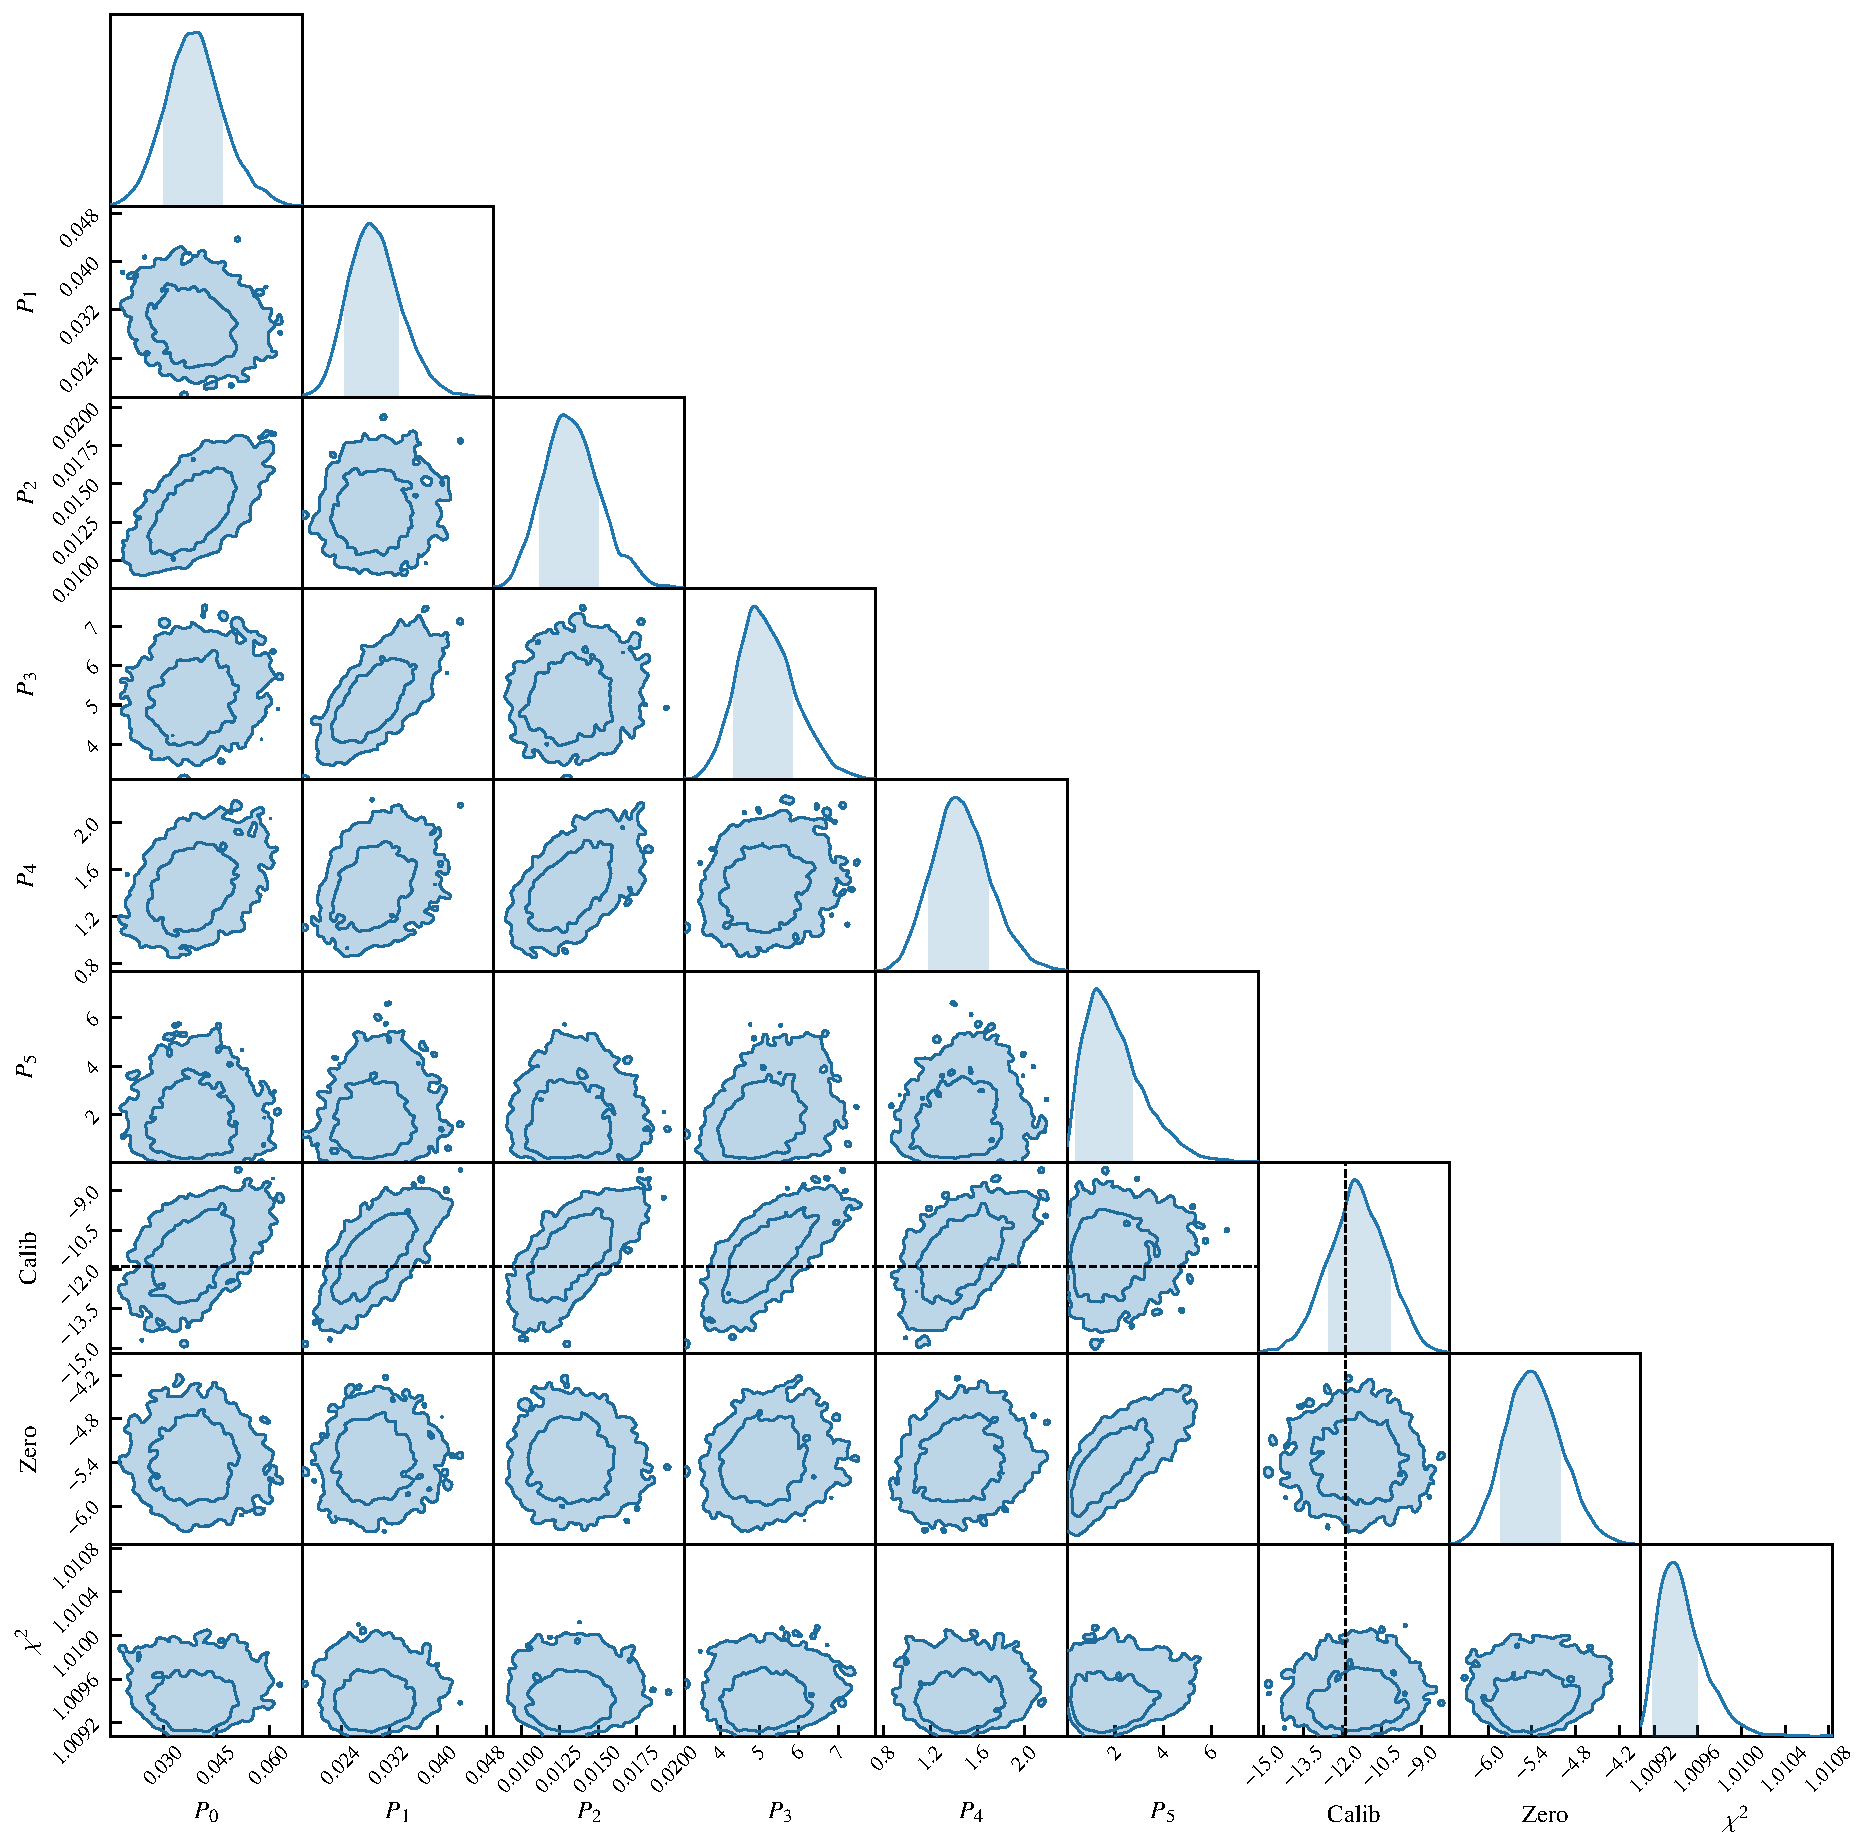
\includegraphics[width=0.95\textwidth]{Figures/Chap_panco/demo_plots/corner.pdf}
    \caption{
        Distribution postérieure dans l'espace des paramètres.
        Les éléments diagonaux représentent les distributions marginalisées sur chacun des paramètres, et les extra-diagonaux les distribution à deux dimensions pour chaque couple de paramètres.
        Les contours représentés sont les intervalles de confiance à $1\sigma$ et $2\sigma$.
        La ligne noire pointillée correspond à la vraie valeur du coefficient de conversion.
    }
    \label{fig:panco2:actlike_corner}
\end{figure*}

\subsubsection{Profils thermodynamiques} % -------------------------------------------- %
Le profil de pression issu de l'analyse est présenté en figure \ref{fig:panco2:actlike_press}.
On voit que le profil de pression mesuré par \texttt{PANCO2} (bleu) est en accord avec la vérité (noir) du lobe de NIKA2 jusqu'au delà de $R_{500}$, ce qui montre le succès de \texttt{PANCO2} pour cet ajustement.
L'interpolation utilisée pour estimer l'incertitude sur le profil de pression est l'interpolation gNFW, décrite en section \ref{sec:panco:interp_np}.
Les résultats des autres méthodes seront discutés par la suite (page \pageref{sec:panco:interp_np_results}).
Comme on peut le voir, le résultat est bien l'interpolation des points non-paramétriques par une fonction lisse: dans ce cas, un tel résultat était attendu, puisque le profil d'entrée est une fonction gNFW.
La matrice de corrélation entre les points du profil de pression est également représentée.
Celle-ci permet d'évaluer l'interdépendance des points du profil de pression, afin de déterminer si la distribution des rayons considérés pour le modèle est adaptée aux données.
Deux points trop proches seront en général fortement anti-corrélés, traduisant le fait que pour deux points très proches, augmenter l'un revient à diminuer l'autre.
La matrice de corrélation sera utilisée pour déterminer la distribution radiale optimale pour des amas synthétiques en section \ref{sec:panco:binning}.

\begin{figure*}[t]
    \centering
    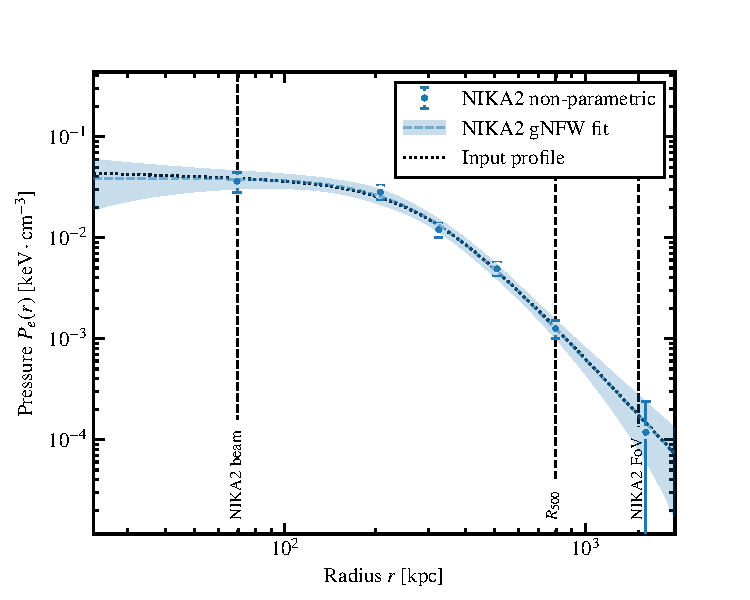
\includegraphics[height=7.25cm, trim={0cm 0cm 1cm 0cm}, clip]{Figures/Chap_panco/demo_plots/pressure.pdf}
    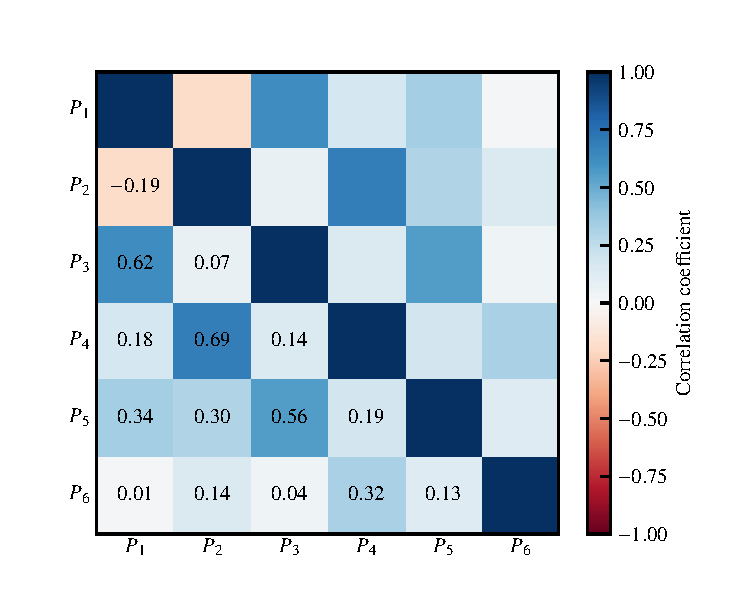
\includegraphics[height=7.25cm, trim={1cm 0cm 0cm 0cm}, clip]{Figures/Chap_panco/demo_plots/pressure_correlations.pdf}
    \caption{
        \textbf{Gauche:} Profil de pression obtenu avec \texttt{PANCO2}.
        Les points bleus représentent le meilleur ajustement en non-paramétrique.
        L'enveloppe bleue représente l'incertitude sur ce profil obtenue par interpolation gNFW des résultats non-paramétriques.
        La courbe pointillée noire est le profil de pression utilisé pour générer la carte de l'amas.
        \textbf{Droite:} Matrice de corrélation entre les points du profil de pression, obtenue à partir des chaînes de Markov.
    }
    \label{fig:panco2:actlike_press}
\end{figure*}

Comme nous le verrons au chapitre suivant, \act\ a été observé par \textit{XMM-Newton}, et ces observations permettent d'extraire un profil de densité (représenté en figure \ref{fig:act:xmm}).
Puisque le profil de pression utilisé pour générer la carte NIKA2 est celui obtenu par ajustement des observations NIKA2 de l'amas réel, nous pouvons combiner ce profil de densité avec le profil de pression mesuré par \texttt{PANCO2} pour représenter les propriétés thermodynamiques de cet amas synthétique.
La procédure employée est décrite en \mypageref{sec:panco:thermo_profiles_x}.
Les profils obtenus par cette combinaison sont représentés en figure \ref{fig:panco2:actlike_thermo}.
On y trouve les profils de température et d'entropie du milieu intra-amas, ainsi que le profil de masse hydrostatique.
Les points bleus représentent les profils obtenus en non-paramétrique.
Comme pour le profil de pression, les enveloppes sont obtenues par interpolation gNFW, ce qui permet d'avoir un profil de masse continu.

\begin{figure*}[t]
    \centering
    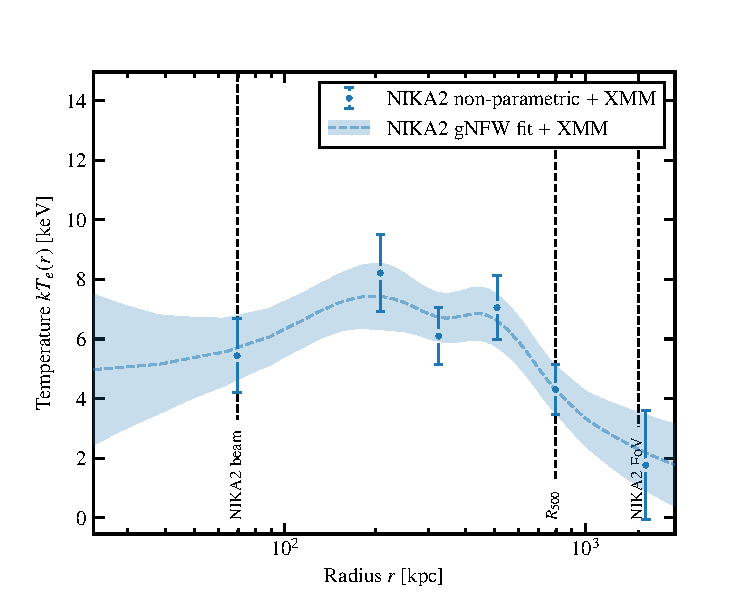
\includegraphics[height=7.2cm, trim={0cm 0cm 1cm 0cm}, clip]{Figures/Chap_panco/demo_plots/temperature.pdf}
    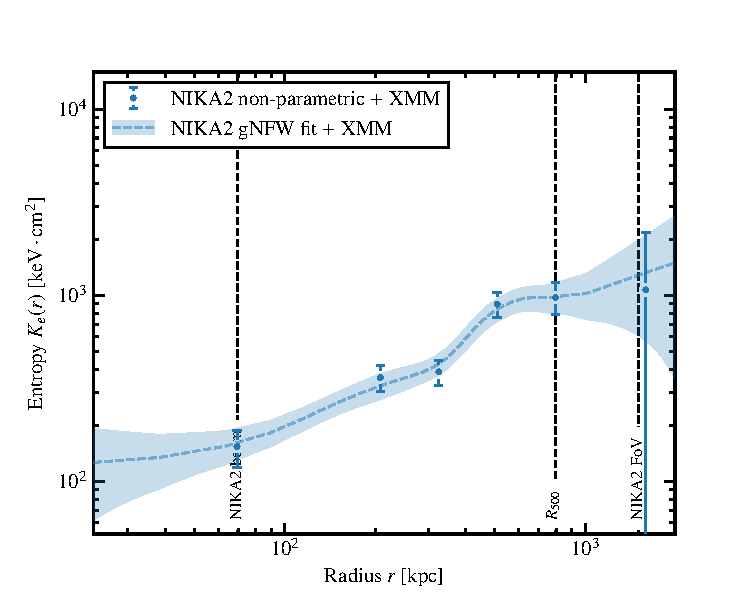
\includegraphics[height=7.2cm, trim={0cm 0cm 1cm 0cm}, clip]{Figures/Chap_panco/demo_plots/entropy.pdf} \\
    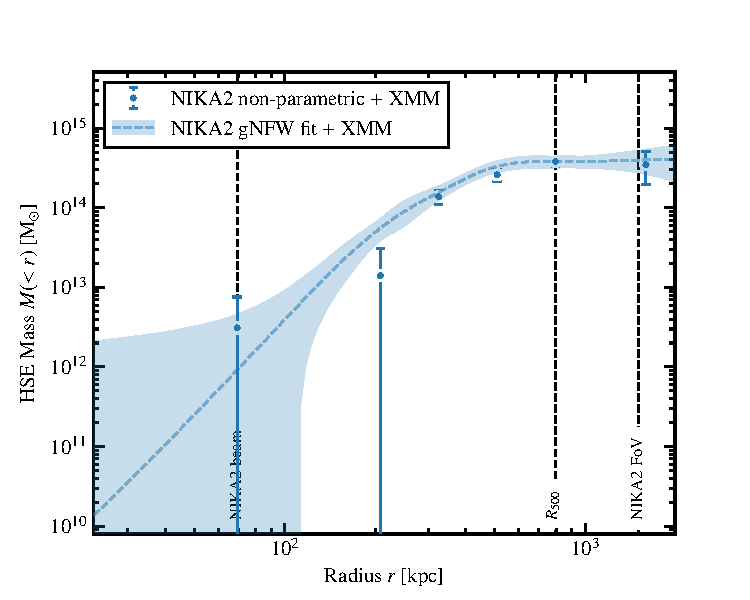
\includegraphics[height=7.2cm]{Figures/Chap_panco/demo_plots/mass.pdf}
    \caption{
        Profils de température (\textit{haut gauche}), d'entropie (\textit{haut droit}), et de masse hydrostatique (\textit{bas}) obtenus par combinaison du profil de pression ajusté par \texttt{PANCO2} et du profil de densité mesuré en X pour \act.
        Les points bleus représentent la combinaison du meilleur ajustement du profil de pression en non-paramétrique avec le profil de densité mesuré en X.
        Les enveloppes bleues représentent l'incertitude sur ces profils obtenue par interpolation gNFW des résultats non-paramétriques.
    }
    \label{fig:panco2:actlike_thermo}
\end{figure*}

\subsubsection{Effet de la méthode d'interpolation} % --------------------------------- %
\label{sec:panco:interp_np_results}
Les résultats trois interpolations possibles pour le profil de pression, présentées en section \ref{sec:panco:interp_np}, sont présentées en figure \ref{fig:panco:interp_np}.
Les profils de masse correspondants sont également représentés.
Les résultats des trois méthodes sont similaires.
Dans les différences notables, on note une discontinuité dans le profil de masse à $r \simeq 300 \;\unit{kpc}$ pour l'interpolation non-paramétrique, due à la nature discontinue de ce modèle.
On observe également une incompatibilité entre les profils interpolés en \textit{splines} et les autres méthodes dans le centre de l'amas ($r \lesssim 100 \;\unit{kpc}$).
Au-delà de $400 \;\unit{kpc}$, les trois méthodes sont en excellent accord.
Le rayon caractéristique $R_{500}$ de cet amas étant de l'ordre de $800 \;\unit{kpc}$, cette similarité traduit un accord entre les trois méthodes pour l'estimation de la masse caractéristique $M_{500}$.
Le choix de la méthode d'interpolation dépend donc des objectifs scientifiques de l'analyse: la détection de surpressions locales nécessitera une interpolation en loi de puissance, alors que l'interpolation par un profil gNFW sera plus adaptée à l'étude d'un profil de masse continu dans le coeur de l'amas.

\begin{figure*}[t]
    \centering
    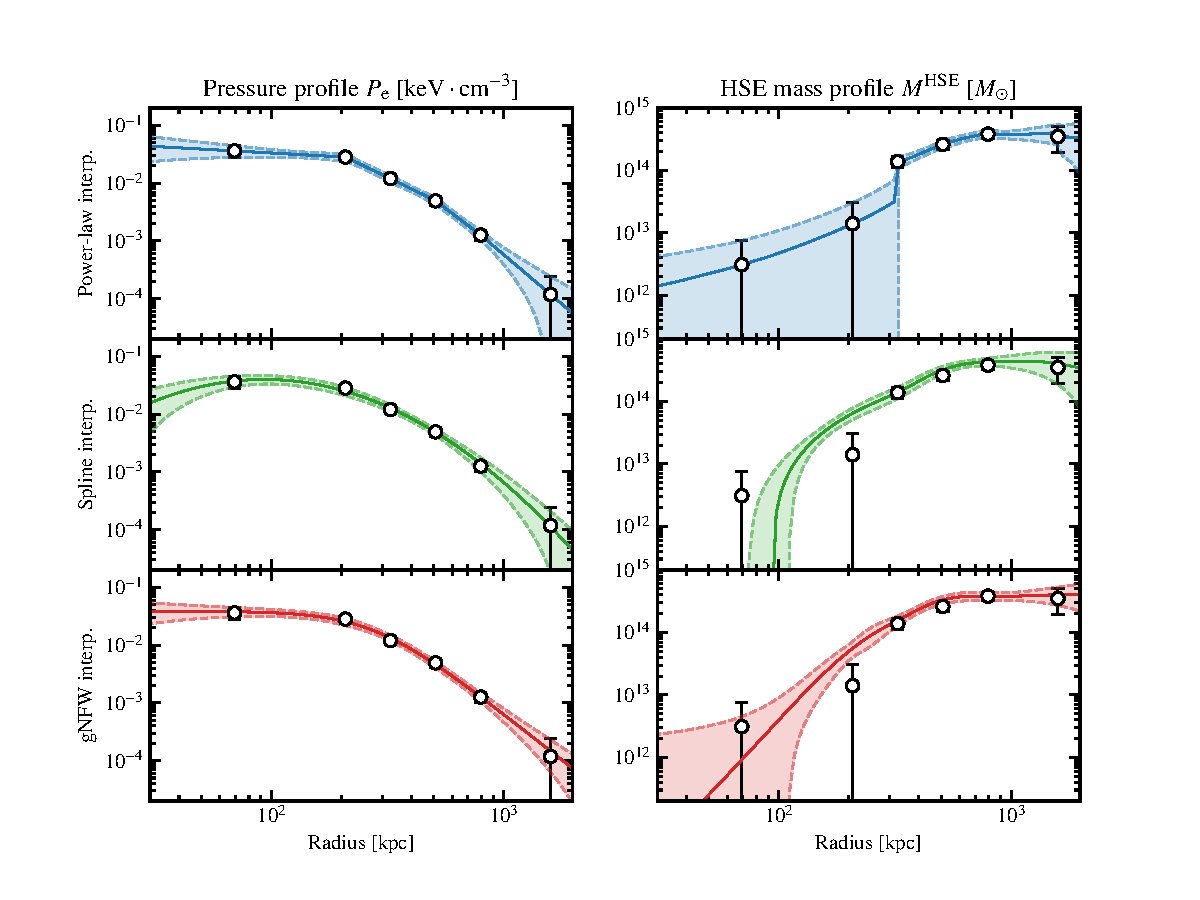
\includegraphics[width=.95\linewidth]{Figures/Chap_panco/demo_plots/interps.pdf}
    \caption{
        \textbf{Gauche:} Interpolations possible du profil de pression non-paramétrique (points blancs) pour un amas simulé: interpolation en loi de puissance (bleu), en \textit{splines} (vert), et en gNFW (rouge).
        La ligne continue montre le profil correspondant à l'interpolation du profil de pression ajustant le mieux les données
        \textbf{Droite:} Profils de masse hydrostatique obtenus par combinaison des profils de pression SZ et de densité X pour les trois méthodes d'interpolation.
        La ligne continue montre le profil correspondant au profil de masse obtenu à partir du profil de pression interpolé à partir du meilleur ajustement.
        Les régions colorées correspondent aux intervalles de confiance à $1\sigma$ sur les profils.
    }
    \label{fig:panco:interp_np}
\end{figure*}

\subsubsection{Grandeurs caractéristiques intégrées} % -------------------------------- %
Enfin, la combinaison des données X et SZ permet, à travers le profil de masse hydrostatique, de calculer les grandeurs intégrées caractéristiques de l'amas.
La procédure utilisée est décrite en \mypageref{sec:panco:integrated_qties}.
La distribution de probabilité obtenue par l'application de cette procédure à l'issue de l'ajustement de l'amas synthétique avec \texttt{PANCO2} est présentée en figure \ref{fig:panco2:actlike_integ}.
On y voit la forte corrélation entre les paramètres, de l'ordre de 80\% pour $R_{500}-Y_{500}$ et $M_{500}-Y_{500}$, et 95\% pour $R_{500}-M_{500}$ (qui sont calculés à partir du même profil de masse).
La distribution dans le plan $M_{500}-Y_{500}$ pour chaque amas du LPSZ est une donnée d'entrée pour l'ajustement de la relation d'échelle $Y_{500}-M_{500}$, discutée au chapitre \ref{chap:scaling}.

\begin{figure*}[t]
    \centering
    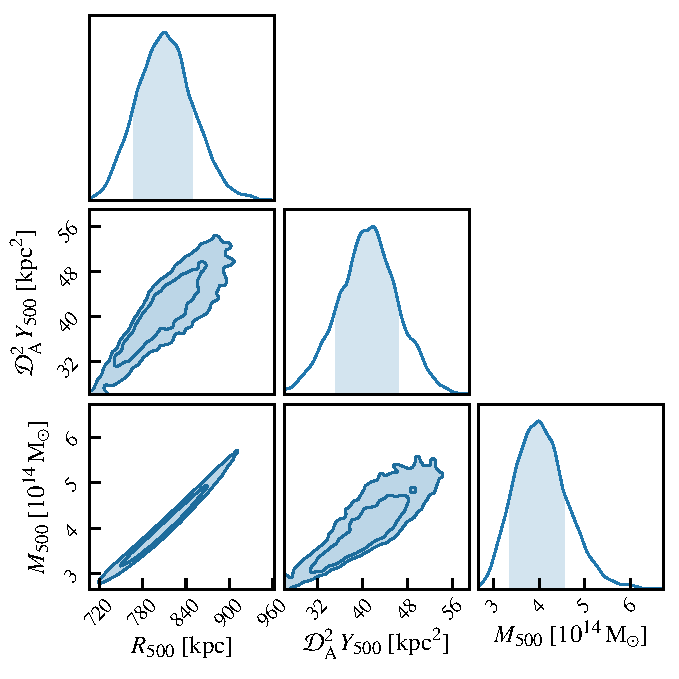
\includegraphics[width=.6\linewidth]{Figures/Chap_panco/demo_plots/integrated_values.pdf}
    \caption{
        Distributions des grandeurs caractéristiques intégrées $R_{500}$, $Y_{500}$, et $M_{500}$ obtenues par l'ajustement avec \texttt{PANCO2} de la carte simulée d'un amas synthétique.
        Les distributions présentées sont les distributions marginalisées à une dimension (éléments diagonaux) et à deux dimensions (éléments extra-diagonaux).
        Les contours présentés sont les intervalles de confiance à $1\sigma$ et $2\sigma$.
    }
    \label{fig:panco2:actlike_integ}
\end{figure*}

% ------------------------------------------------------------------------------------ %
\subsection{Optimisation de la distribution radiale} \label{sec:panco:binning}

Deux amas synthétiques considérés comme extrêmes pour le grand programme SZ ont été étudiés: un amas compact C1, de basse masse et haut redshift; et un amas étendu C2, de grande masse et bas redshift:
\begin{align}
    \label{eq:panco:synth_clusters}
    \nonumber \text{C1}: \; M_{500} = 3.5 \times 10^{14} \; M_\odot, \; z=0.9 ; \\
              \text{C2}: \; M_{500} = 9.5 \times 10^{14} \; M_\odot, \; z=0.5 .
\end{align}
Les propriétés thermodynamiques de ces amas ont été simulées en considérant une symétrie sphérique, et un profil de pression universel tel que mesuré par \myciteauthor{arnaud_universal_2010}.
Comme pour l'étude précédente, des cartes NIKA2 de ces amas sont simulées par intégration le long de la ligne de visée, conversion, filtrage par le lobe et par une fonction de transfert réaliste, puis ajout de bruit blanc réaliste.

Les cartes des amas C1 et C2 ont ensuite été utilisées afin d'optimiser le \textit{binning} du profil de pression, c'est-à-dire le choix des rayons $R_i$ considérés dans le modèle non-paramétrique de l'équation (\ref{eq:panco:nonparam}).
Ainsi, chacune de ces cartes a été ajustée pour plusieurs \textit{binning} différents, définis comme suit:
\begin{itemize}[leftmargin=*]
    \setlength\itemsep{0pt}
    \item Le premier rayon $R_0$ correspond à la demi-largeur à mi-hauteur (HWHM) du lobe de NIKA2, rayon en dessous duquel toute fluctuation de signal est lissée par la résolution de l'instrument;
    \item $n$ points sont ensuite ajoutés, espacés logarithmiquement entre $3 \times R_0$ et le rayon $R_{500}$ de l'amas ;
    \item Un dernier point à $2 \times R_{500}$ pour contraindre la pente externe du profil de pression.
\end{itemize}
L'ajustement est réalisé avec \texttt{PANCO2} sur les deux cartes d'amas simulées entre $n=2$ et $n=10$ dans le but de trouver la valeur de $n$ la plus adaptée aux amas du grand programme SZ.
Le choix du meilleur $n$ est basé sur deux critères.
Le profil de pression reconstruit par \texttt{PANCO2} doit être aussi proche que possible du profil réel utilisé en entrée de la simulation; et la corrélation entre deux points successifs du profil de pression $(P_i, P_{i+1})$ doit être minimale, symbolisant des mesures indépendantes du profil de pression à différents rayons.

Les résultats sont représentés sur la figure \ref{fig:panco:binning}.
Ils montrent qu'un amas étendu peut être modélisé avec un plus grand nombre de rayons qu'un amas compact, puisque l'extension de l'amas est plus grande par rapport au lobe de NIKA2 et dispose d'une meilleure couverture angulaire.
Pour l'amas compact C1, on voit qu'il est raisonnable de considérer jusqu'à $n=6$ points entre trois fois la demi-largeur à mi-hauteur du lobe de NIKA2 et le rayon caractéristique $R_{500}$ de l'amas avant que les résultats ne diffèrent grandement de la vérité.
D'autre part, on observe que la corrélation moyenne entre deux mesures de pressions successives augmente rapidement à partir de $n=4$.
Pour l'amas C2, les conclusions sont similaires: la justesse des résultats ne se dégrade que graduellement avec $n$, mais la corrélation entre deux points successifs augmente à partir de $n=5$.
Ces conclusions nous montrent que, quel que soit le critère choisi, les valeurs de $n$ optimales pour les amas les plus étendus et les plus compacts du grand programme SZ ne sont différentes que d'un point.
Par la suite, nous choisirons $n=5$, apparaissant comme la plus grande valeur utilisable avant que la corrélation des mesures de pression ne dépasse les 50\% pour les amas les plus compacts du programme.

\begin{SCfigure*}[][t]
    \caption{%
        Influence du nombre de rayons considérés dans le modèle non-paramétrique sur les résultats de \texttt{PANCO2}.
        $n$ est le nombre de points situés entre trois fois la demi-largeur à mi-hauteur du lobe de NIKA2 et le rayon caractéristique $R_{500}$ de l'amas (inclus).
        Les amas considérés sont des amas synthétiques ayant un profil de pression universel, considérant un amas compact (C1, bleu) et un amas étendu (C2, rouge) pour le grand programme SZ de NIKA2 (équation \ref{eq:panco:synth_clusters}).
        Le panneau du \textit{haut} représente l'évolution de la différence relative entre le résultat de \texttt{PANCO2} et la vérité intégré sur la plage de rayons considérés dans le modèle.
        Le panneau du \textit{bas} représente l'évolution de la corrélation moyenne entre deux points successifs du profil de pression.
    }
    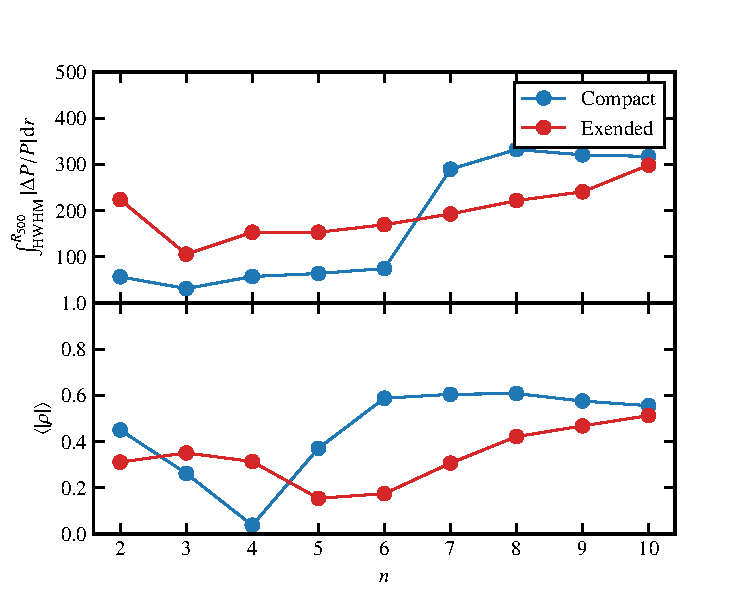
\includegraphics[height=8cm]{Figures/Chap_panco/evol.pdf}
    \label{fig:panco:binning}
\end{SCfigure*}

% ------------------------------------------------------------------------------------ %
\subsection{La simulation MUSIC et l'échantillon jumeau du grand programme SZ}
\label{sec:panco:music}

La simulation MUSIC (\textit{Marenostrum-MultiDark SImulations of galaxy Clusters}, \cite{sembolini_music_2013}) est une simulation hydrodynamique d'amas de galaxies.
Elle est basée sur la technique de la resimulation par \textit{zoom-in} \cite{klypin_resolving_2001}, dont le principe de fonctionnement est rappelé ici.
Une simulation cosmologique à $N$-corps à relativement basse résolution  est réalisée pour simuler l'évolution de l'Univers, à partir de conditions initiales à haut redshift jusqu'à $z=0$.
Les résultats de cette simulation sont utilisés pour trouver les zones correspondant aux pics de densité de la toile cosmique formée, régions qui abritent les amas de galaxies dans l'Univers.
Ces régions sont ensuite resimulées, en repartant des mêmes conditions initiales, mais en ne considérant qu'un plus petit volume, correspondant à la région de l'amas seulement, ce qui diminue le temps nécessaire à la production des simulations.
Cette diminution de volume permet donc d'ajouter des ingrédients à la simulation, comme de la nouvelle physique, ainsi qu'un plus grand nombre de particules, augmentant ainsi la résolution finale de la simulation.

Dans le cas de MUSIC, les simulations d'entrée sont \textit{Marenostrum} \cite{gottlober_shape_2007} et \textit{MultiDark} \cite{prada_halo_2012}.
Un total d'environ 500 halos sont resimulés en incluant des phénomènes hydrodynamiques, de transfert radiatif et de formation stellaire.
Les amas resimulés offrent donc une physique bien plus riche que les halos d'origine, en plus d'une résolution un ordre de grandeur plus élevée.
Chaque amas est resimulé à partir de conditions initiales à un redshift $z=9$ jusqu'à $z=0$, et des \textit{snapshots} sont enregistrés à plusieurs redshifts intermédiaires afin de pouvoir étudier l'évolution des amas au cours du processus de formation des structures.

L'échantillon considéré pour la validation de \texttt{PANCO2} est un sous-ensemble de l'échantillon MUSIC sélectionné pour être similaire à l'échantillon du grand programme SZ de NIKA2.
Cet échantillon, créé par \myciteauthor{ruppin_impact_2019-1}, comporte 32 amas, couvrant une gamme de masse similaire à celle couverte par le grand programme SZ, à des redshifts de 0.54 et 0.82.
Les amas ont été sélectionnés afin d'avoir autant d'amas morphologiquement relaxés que d'amas perturbés.
Cet échantillon est particulièrement adapté à la validation de \texttt{PANCO2} : il est composé d'amas réalistes similaires à ceux du grand programme SZ de NIKA2.
Des observations NIKA2 simulées sont produites pour ces amas selon la procédure décrite dans \cite{ruppin_impact_2019-1}.
La pression -- connue -- du milieu intra-amas est intégrée le long d'une ligne de visée arbitraire afin d'obtenir une carte de paramètre de Compton, qui est ensuite convertie en unités de brillance de surface.
Celle-ci est ensuite convoluée par le lobe instrumental de NIKA2 et par une fonction de transfert fiducielle réaliste, et une réalisation de bruit corrélé est ajoutée suivant un spectre de puissance de bruit réaliste.
Les cartes résultantes sont donc des simulations réalistes d'observations avec NIKA2 des amas de l'échantillon.
Elles sont représentées sur la figure \ref{fig:panco:all_maps_music}.
On remarque une grande variété dans les morphologies d'amas, ainsi que dans le rapport signal sur bruit des observations.

\begin{figure*}[t]
    \centering
    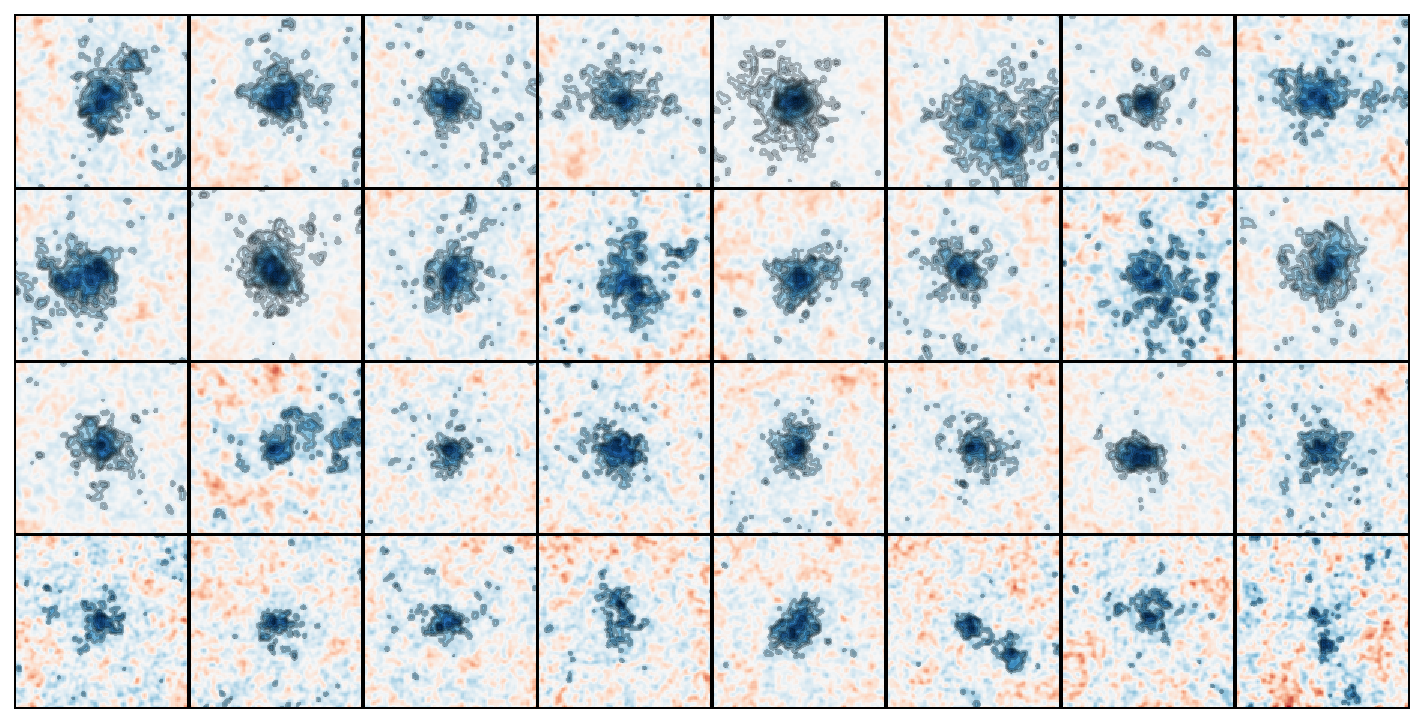
\includegraphics[width=\linewidth]{Figures/Chap_panco/all_maps_music.pdf}
    \caption{Cartes simulées des 32 amas de l'échantillon utilisé pour la validation du code.
        Les échelles de couleurs sont arbitraires.
        Chaque carte est représentée dans un carré de 6.5' de coté, centré aux coordonnées du pic de densité du halo considéré.
        Les contours représentent les niveaux de signal sur bruit commençant à $3\sigma$ espacés de $1\sigma$.
        Les cartes sont lissées par un noyau gaussien de largeur à mi-hauteur 10''  pour des raisons visuelles.
    }
    \label{fig:panco:all_maps_music}
\end{figure*}

% ------------------------------------------------------------------------------------ %
\subsection{Ajustement du profil de pression} \label{sec:music_pressure}

Le profil de pression de chacun des amas de l'échantillon est estimé à l'aide de \texttt{PANCO2}.
Un modèle non-paramétrique est considéré : les profils de pression des amas MUSIC étant réalistes, toutes leurs caractéristiques ne peuvent pas être capturées par un modèle gNFW, rendant la comparaison d'un profil de pression ajusté par un tel modèle au vrai profil inappropriée.
Nous choisissons le même \textit{binning} que celui décrit dans la section \ref{sec:panco:binning} avec $n=5$ points entre la résolution de NIKA2 et $R_{500}$.
La fonction de transfert et la matrice de covariance du bruit utilisées pour générer les cartes simulées sont considérées dans l'analyse.

\begin{figure*}[p]
    \centering
    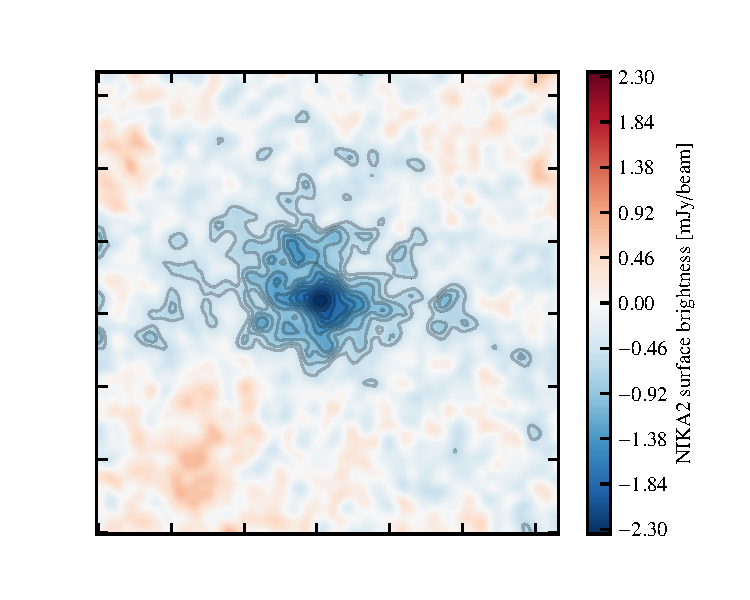
\includegraphics[height=6.5cm, trim={1.4cm 0.5cm 0.8cm 1.0cm}, clip]{Figures/Chap_panco/profiles_music/Bin1_cl00024_map.pdf} \hspace{10pt}
    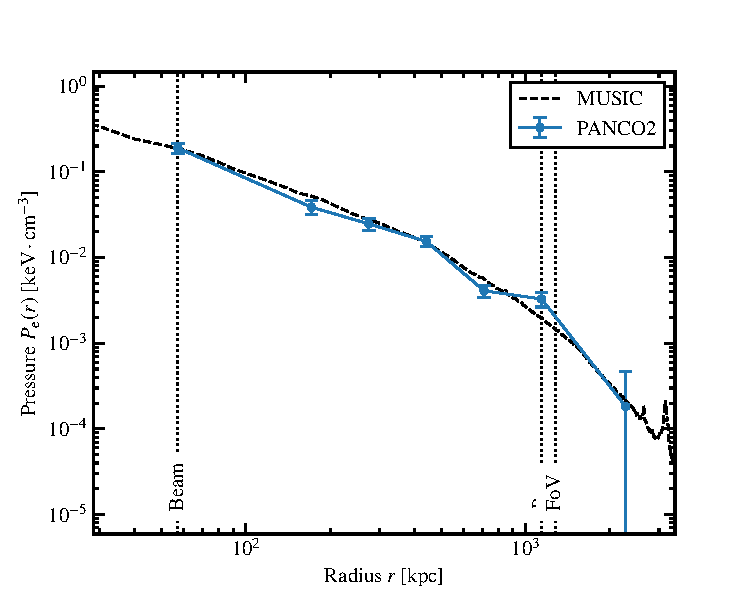
\includegraphics[height=6.5cm, trim={0cm 0cm 1cm 1.0cm}, clip]{Figures/Chap_panco/profiles_music_2/00024.0.54.pdf}
    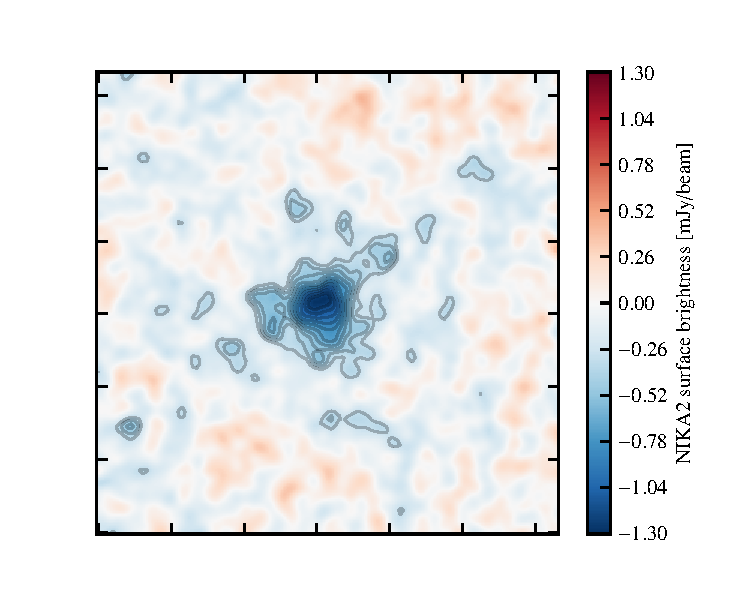
\includegraphics[height=6.5cm, trim={1.4cm 0.5cm 0.8cm 1.0cm}, clip]{Figures/Chap_panco/profiles_music/Bin1_cl00032_map.pdf} \hspace{10pt}
    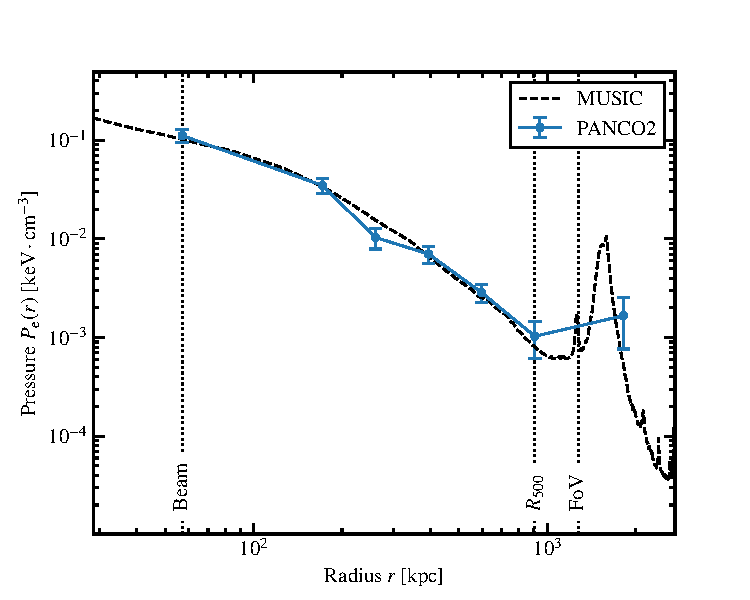
\includegraphics[height=6.5cm, trim={0cm 0cm 1cm 1.0cm}, clip]{Figures/Chap_panco/profiles_music_2/00032.0.54.pdf}
    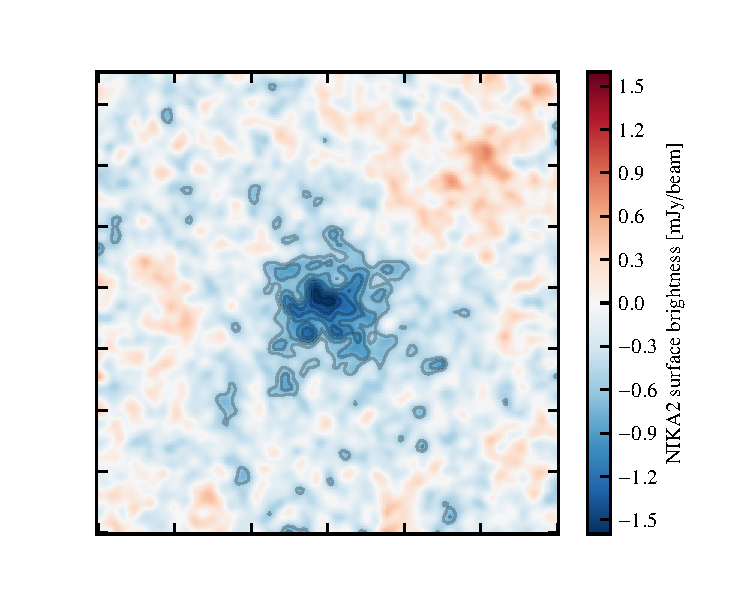
\includegraphics[height=6.5cm, trim={1.4cm 0.5cm 0.8cm 1.0cm}, clip]{Figures/Chap_panco/profiles_music/Bin2_cl00047_map.pdf} \hspace{10pt}
    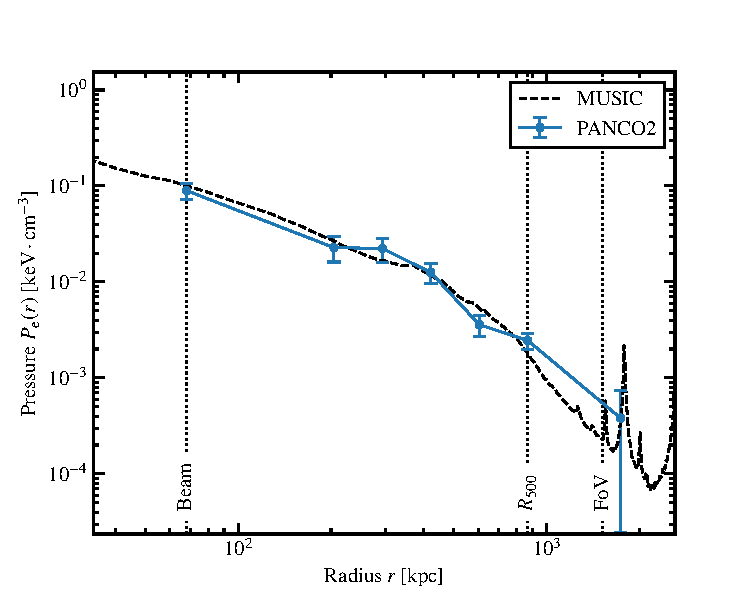
\includegraphics[height=6.5cm, trim={0cm 0cm 1cm 1.0cm}, clip]{Figures/Chap_panco/profiles_music_2/00047.0.82.pdf}
    %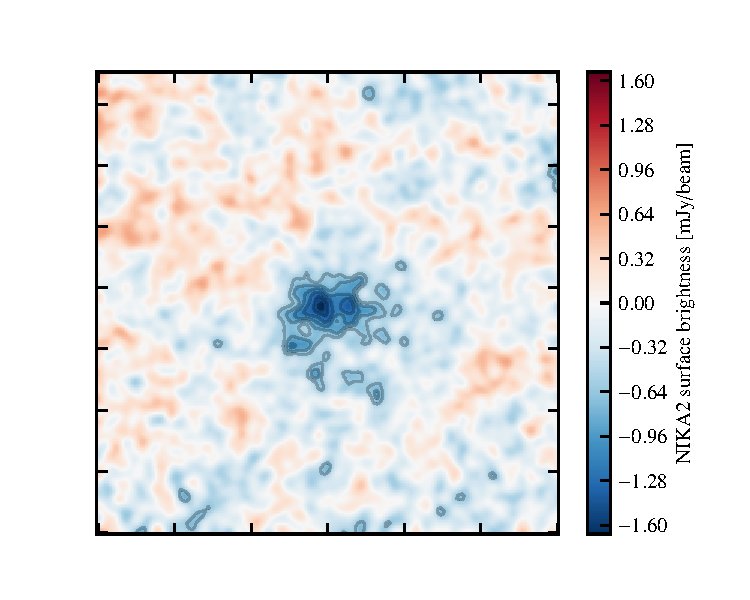
\includegraphics[height=5.75cm, trim={1.4cm 0.5cm 0.8cm 1.0cm}, clip]{Figures/Chap_panco/profiles_music/Bin2_cl00067_map.pdf} \hspace{15pt}
    %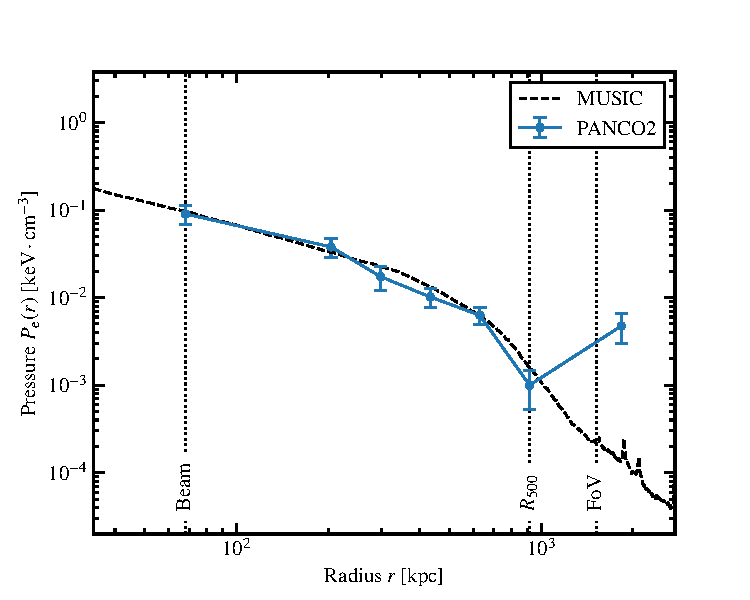
\includegraphics[height=5.75cm, trim={0cm 0cm 1cm 1.0cm}, clip]{Figures/Chap_panco/profiles_music_2/00067.0.82.pdf}
    \caption{Illustration des cartes NIKA2 simulées (\textit{gauche}) et profils de pression mesurés (\textit{droite}) pour trois amas MUSIC: deux à $z=0.54$ (\textit{haut, milieu}) et un à $z=0.82$ (\textit{bas}).
        La légende des cartes est la même que pour la figure \ref{fig:panco:all_maps_music}.
        Les lignes pointillées noires représentent les profils de pression réels des amas tels qu'extraits de la simulation MUSIC.
        Les profils bleus sont ceux obtenus par ajustement avec \texttt{PANCO2}.
        Tous les profils sont centrés sur le pic de potentiel gravitationnel des amas tels que mesurés dans la simulation MUSIC.
    }
    \label{fig:panco:music_profs}
\end{figure*}

La convergence du MCMC est atteinte en environ une à deux heures par amas, représentant un gain d'un facteur $\sim 40$ par rapport à \texttt{PANCO}, qui réalisait l'ajustement des mêmes cartes en deux à trois jours par amas d'après \myciteauthor{ruppin_impact_2019-1}\footnotemark.
\footnotetext{Il est important de préciser que \texttt{PANCO} a été utilisé dans \cite{ruppin_impact_2019-1} pour ajuster simultanément des cartes simulées NIKA2 et \textit{Planck} des amas MUSIC, alors que l'analyse \texttt{PANCO2} décrite ici n'a considéré que les cartes NIKA2.}
Il est à noter qu'en considérant le bruit comme blanc -- c'est à dire en négligeant les éléments extra-diagonaux de la matrice de covariance du bruit -- \texttt{PANCO2} est capable de réaliser l'ajustement en cinq à quinze minutes par amas seulement, soit environ dix fois plus vite.
Ce constat motive grandement la poursuite du travail sur la soustraction du bruit corrélé dans les cartes NIKA2, afin d'obtenir des spectres de puissance de bruit résiduel les plus plats possibles et de pouvoir négliger les corrélations pixel-à-pixel du bruit dans les cartes.
Ce gain de temps permettrait de mener des études systématiques plus approfondies, comme l'évolution des résultats avec le \textit{binning} du profil de pression non-paramétrique sur l'ensemble des données du grand programme SZ de NIKA2.

Les résultats montrent un excellent accord entre les profils mesurés par \texttt{PANCO2} et ceux extraits de la simulation MUSIC.
Trois exemples sont présentés dans la figure \ref{fig:panco:music_profs}, illustrant la compatibilité entre le profil de pression réel et les résultats de \texttt{PANCO2} pour trois des amas de l'échantillon MUSIC.
On y voit un excellent accord dans les barres d'erreur entre les profils de pression ajustés par \texttt{PANCO2} et les données d'entrée sur toute la couverture radiale considérée dans l'ajustement, du lobe de NIKA2 à $2 \times R_{500}$, soit hors du champ de vue pour les amas considérés.
Cet accord permet de conclure que les résultats de \texttt{PANCO2} sont satisfaisants, même lorsque le logiciel est confronté à des données réalistes affectées des bruits et filtrages caractéristiques des observations d'amas avec NIKA2.

% ==================================================================================== %
\section{Conclusions}

L'observation des amas de galaxies du grand programme SZ de NIKA2 permet de mesurer la distribution de pression dans le milieu intra-amas individuellement pour chaque source.
L'approche choisie par la collaboration NIKA2 est le \textit{forward modelling}, permettant une prise en compte des différents phénomènes affectant les observations de l'effet Sunyaev-Zeldovich avec NIKA2.
Ce chapitre a présenté l'algorithme développé pour effectuer ces mesures en utilisant une procédure MCMC pour ajuster un modèle de profil de pression sur les données NIKA2.

Au début de ma thèse, cet algorithme était implémenté dans le logiciel \texttt{PANCO}, alors pipeline officiel du grand programme SZ de NIKA2.
Ce chapitre a présenté le développement de \texttt{PANCO2}, dont l'objectif était la livraison d'un logiciel offrant plus de possibilités d'analyse tout en étant plus rapide.
Le désir d'optimisation du temps d'exécution provenait du fait que \texttt{PANCO} ne permettait l'analyse d'un échantillon de plusieurs dizaines d'amas qu'au prix de plusieurs semaines de calcul, limitant l'exploitation des données du grand programme SZ de NIKA2.
L'analyse de cartes synthétiques d'un échantillon d'amas issus de la simulation hydrodynamique MUSIC a permis à la fois d'affirmer la capacité de \texttt{PANCO2} à estimer correctement le profil de pression d'amas de galaxies à partir de données NIKA2 réalistes, mais également de comparer ses performances à celles de \texttt{PANCO}.
Le temps d'exécution est diminué par un facteur d'environ quarante, rendant possible non seulement l'analyse d'échantillons d'amas en un temps raisonnable, mais également des études systématiques afin de tirer des informations plus fines sur les propriétés du milieu intra-amas à partir des observations NIKA2.
Ceci a mené au choix de \texttt{PANCO2} comme pipeline officiel du grand programme SZ de NIKA2, et à la préparation d'une mise à disposition de \texttt{PANCO2} pour la communauté scientifique.
